\section{Localization in challenging conditions}

\label{sec:results}

\begin{frame}{Dataset for Localization in challenging conditions}
	
	\textcolor{mLightBrown}{\textbf{Dataset:}} we train and test our proposal on RobotCar\footfullcite{Maddern2016} dataset
	
	\textcolor{mLightBrown}{\textbf{Deep architectures:}} Resnet18 or Alexnet encoder combined with NetVLAD or MAC descriptor

	\vfill
	
	\uncover<2->{
		\textcolor{mLightBrown}{\textbf{Competitors:}} Hallucination network\footfullcite{Hoffman2016} \& same descriptor only trained with RGB
	}
	
	\vfill
	
	\uncover<3->{
		\textcolor{mLightBrown}{\textbf{Metric:}} we compare the distance between \textbf{the top ranked} returned database image position and the query ground truth position.
		
	}
\end{frame}

%\begin{frame}{Dataset for Localization in challenging conditions}
%	
%	\begin{minipage}[t]{0.6\linewidth}
%		We test our proposal on RobotCar$^1$ dataset with various localization scenarios and different combination of encoders/descriptors.
%		\vspace{1cm}
%		
%		\uncover<3>{
%		\textbf{Metric:} we compute the distance between \textbf{the top ranked} returned database image position and the query ground truth position and report the percentage of queries well located under a threshold D.
%		}
%	\end{minipage}\hfill
%	\uncover<2->
%	{
%	\begin{minipage}[t]{0.32\linewidth}
%		\textbf{Competitors:}
%		\begin{itemize}
%			\item[\textbf{-{}-{}-}] Only RGB [RGB]
%			\item[\textbf{-x-}] Hallucination network$^2$ [RGBtD (Hall)]
%			\item[\textbf{-o-}] Our proposal [RGBtD (our)]
%		\end{itemize}
%	\end{minipage}
%	\textcolor{white}{\footfullcite{Maddern2016}\footfullcite{Hoffman2016}}	
%	}	
%\end{frame}

%
%\begin{frame}{Results: cross-season localization}
%	\scriptsize
%	\begin{tabularx}{1.08\linewidth}{X X X X X}
%		Query & NetVLAD (our) & NetVLAD & MAC (our) & MAC \\
%	\end{tabularx}
%	\fboxsep=1pt%padding thickness
%	\fboxrule=1pt
%
%	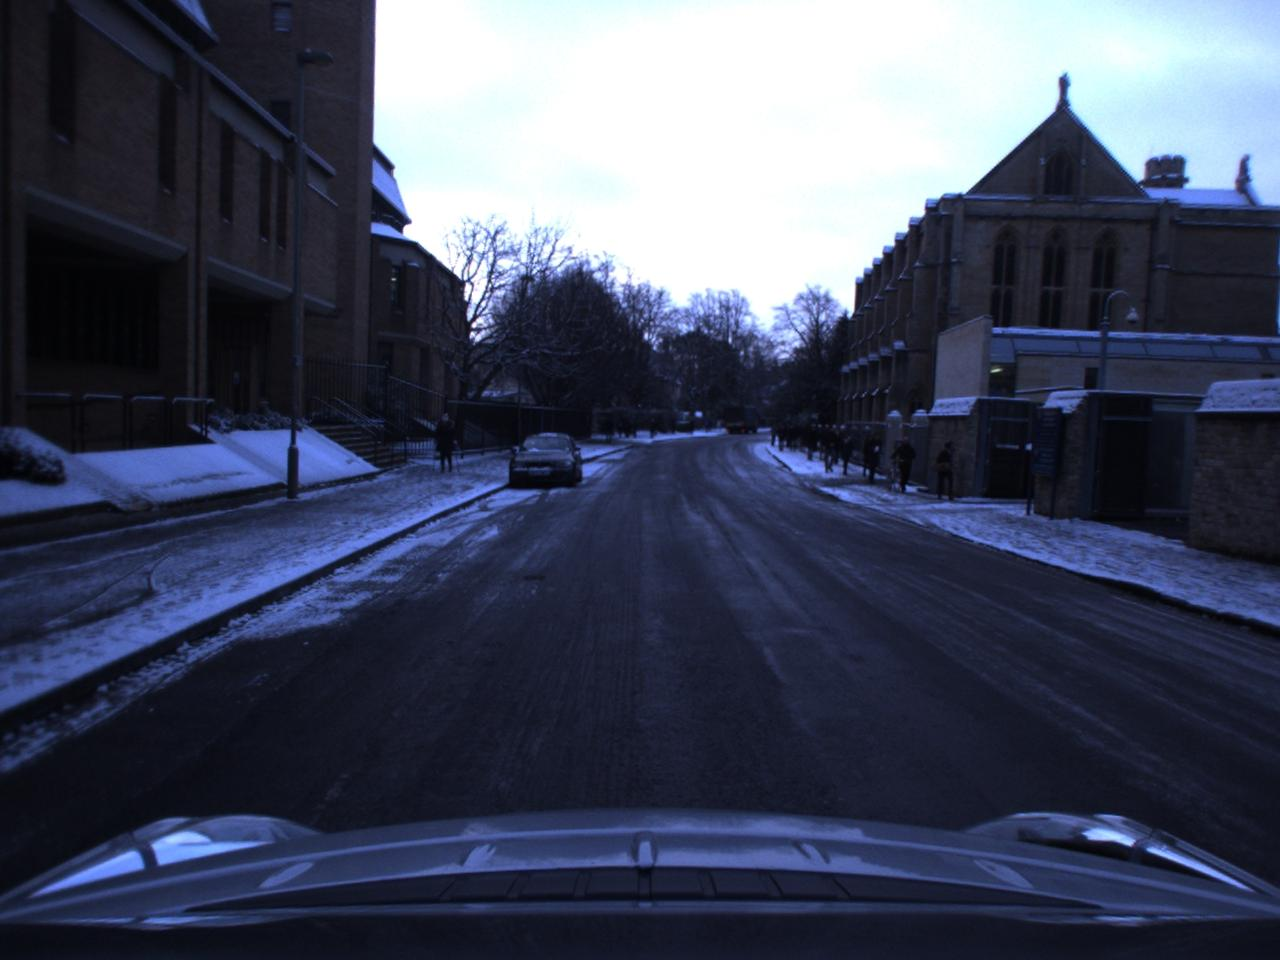
\includegraphics[width=0.12\linewidth]{ims_res/snow/q1/Q.jpg}\hfill
%	\fcolorbox{green}{green}{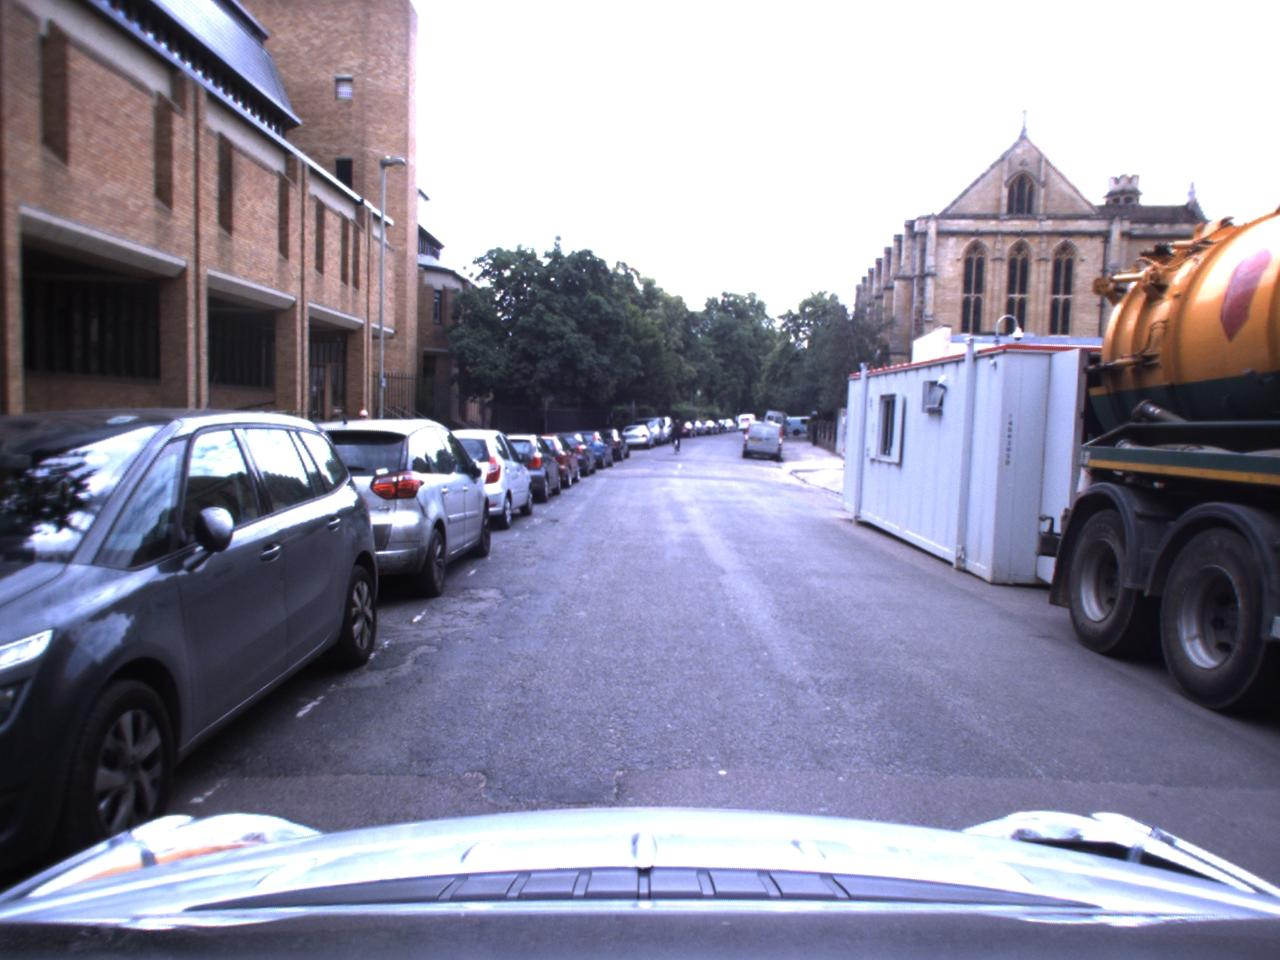
\includegraphics[width=0.12\linewidth]{ims_res/snow/q1/NetVLAD_our.jpg}}\hfill
%	\fcolorbox{red}{red}{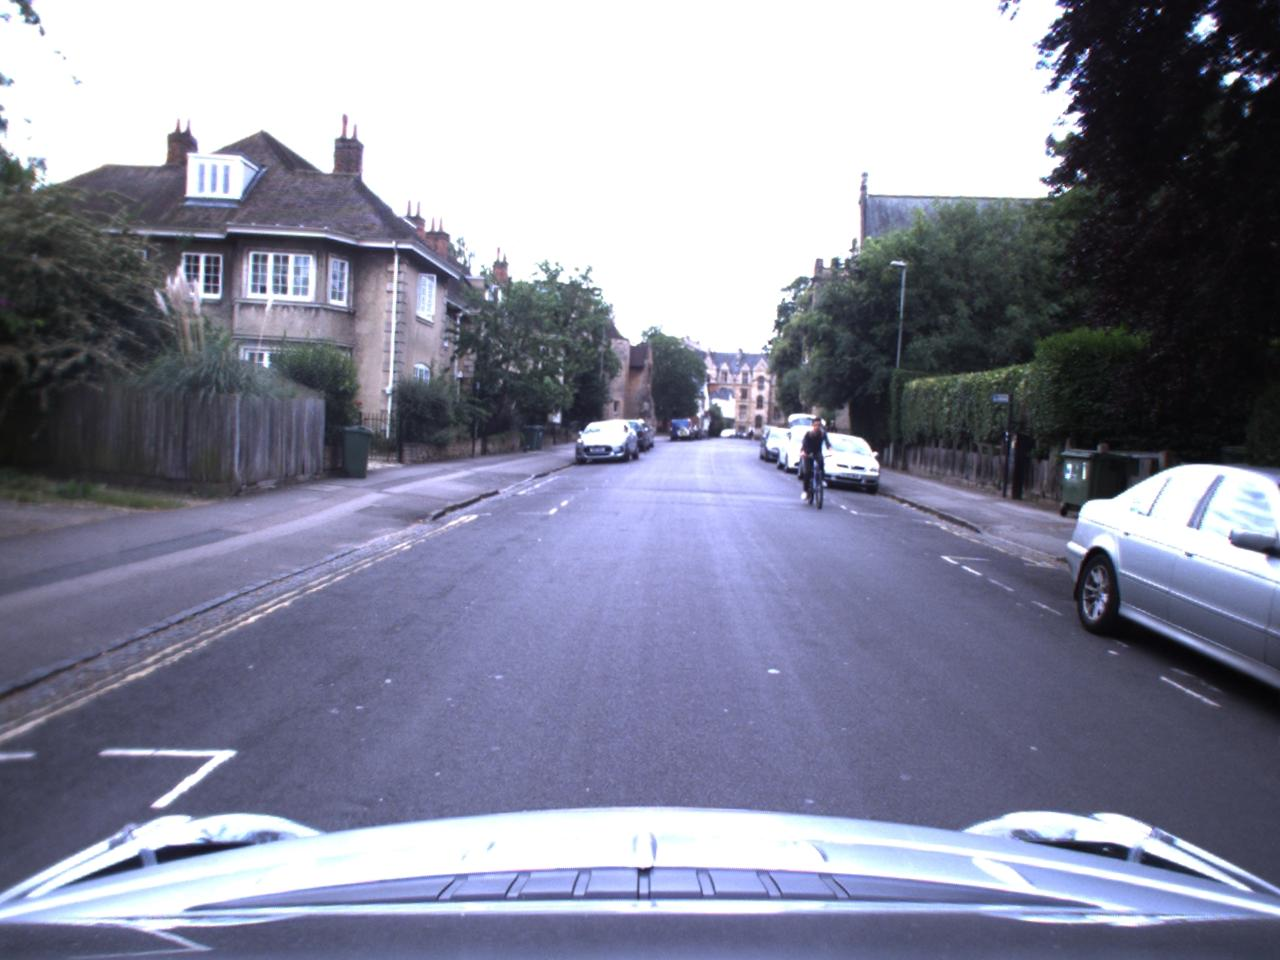
\includegraphics[width=0.12\linewidth]{ims_res/snow/q1/NetVLAD.jpg}}\hfill
%	\fcolorbox{red}{red}{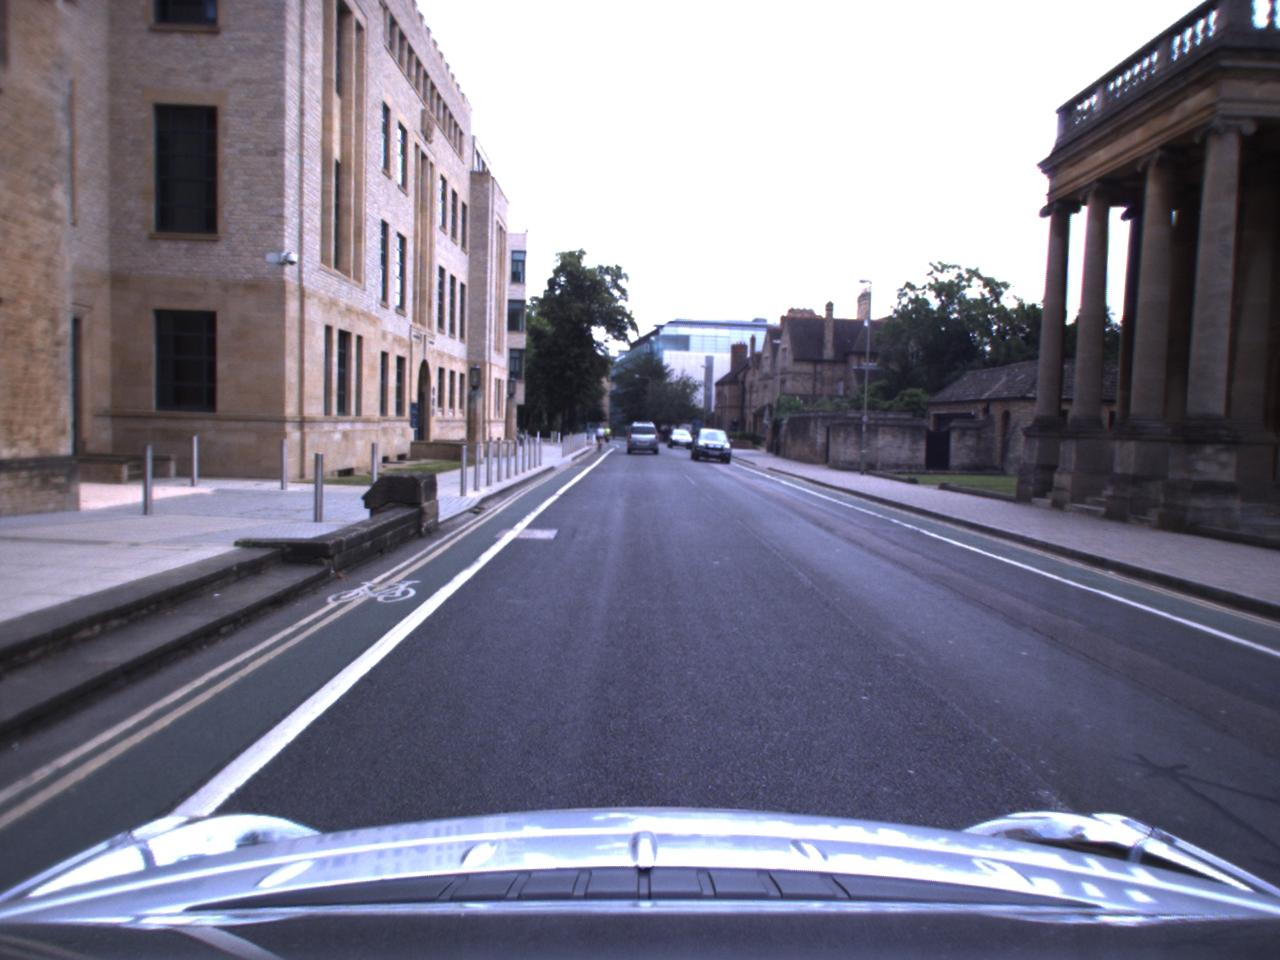
\includegraphics[width=0.12\linewidth]{ims_res/snow/q1/MAC_our.jpg}}\hfill
%	\fcolorbox{red}{red}{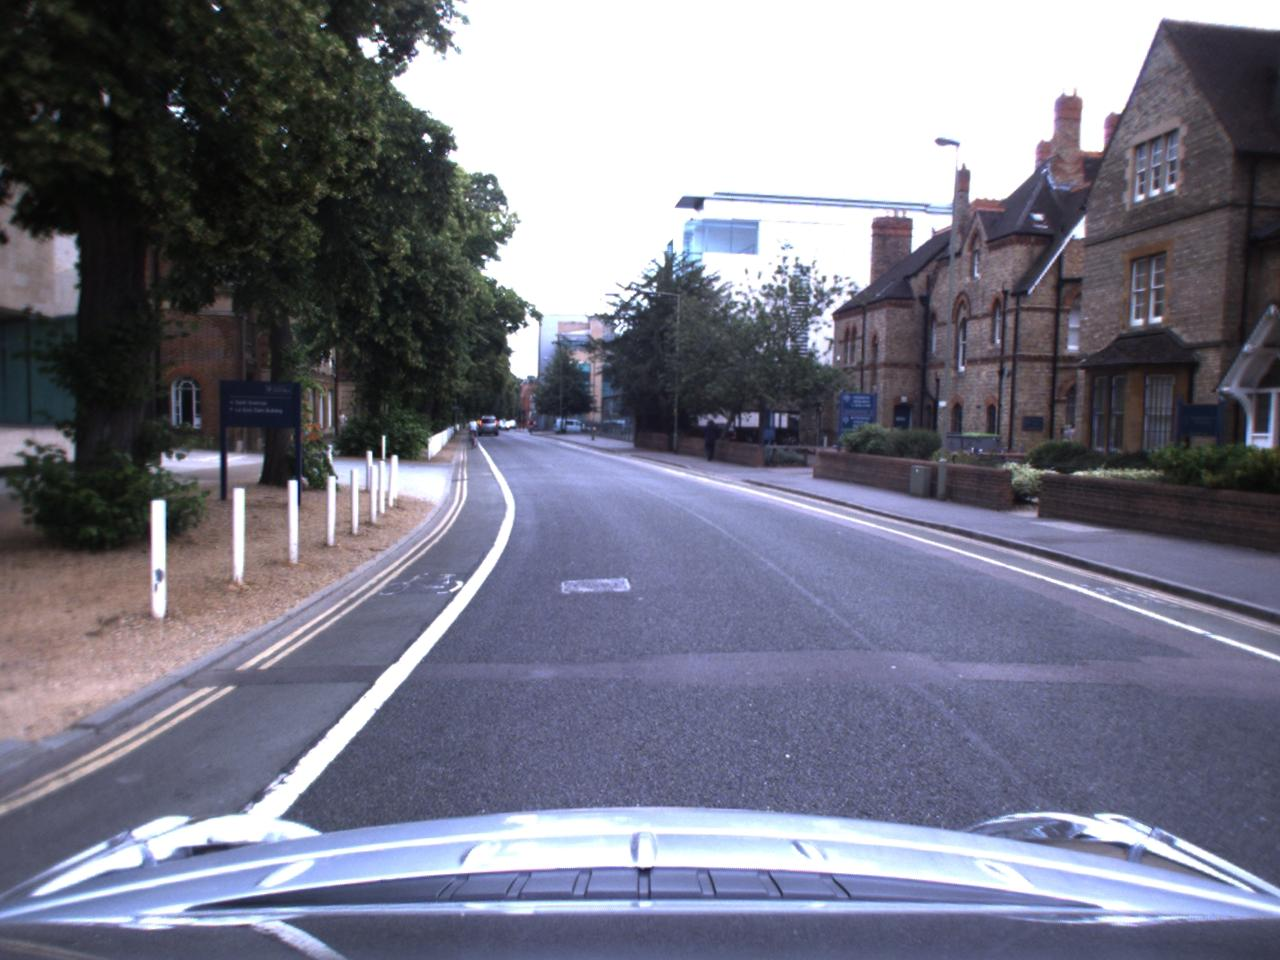
\includegraphics[width=0.12\linewidth]{ims_res/snow/q1/MAC.jpg}}
%	
%	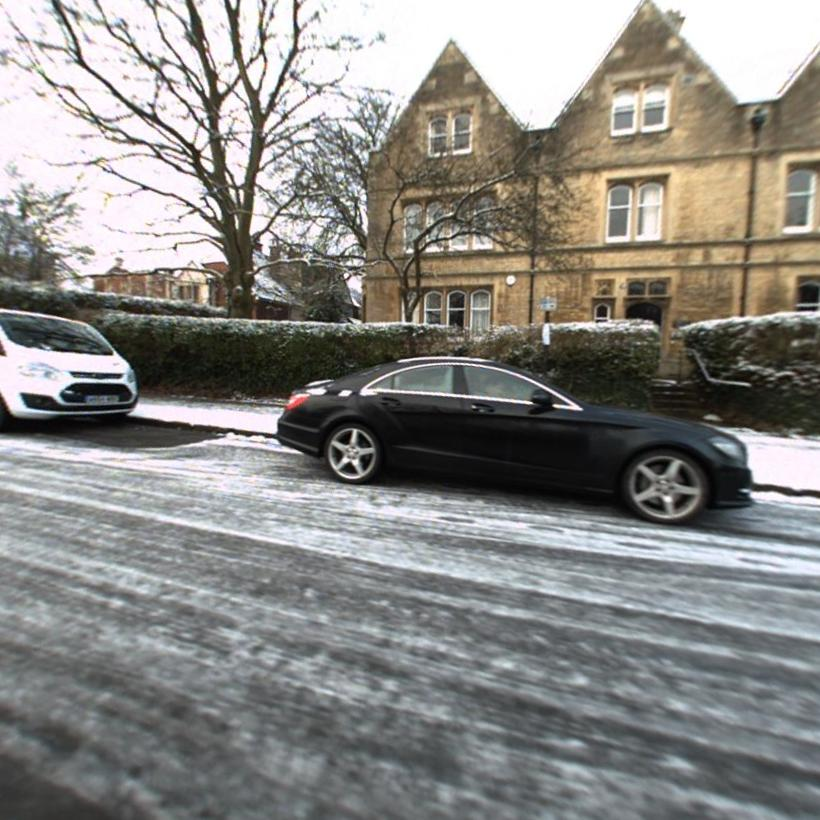
\includegraphics[width=0.12\linewidth]{ims_res/snow/q2/Q.jpg}\hfill
%	\fcolorbox{green}{green}{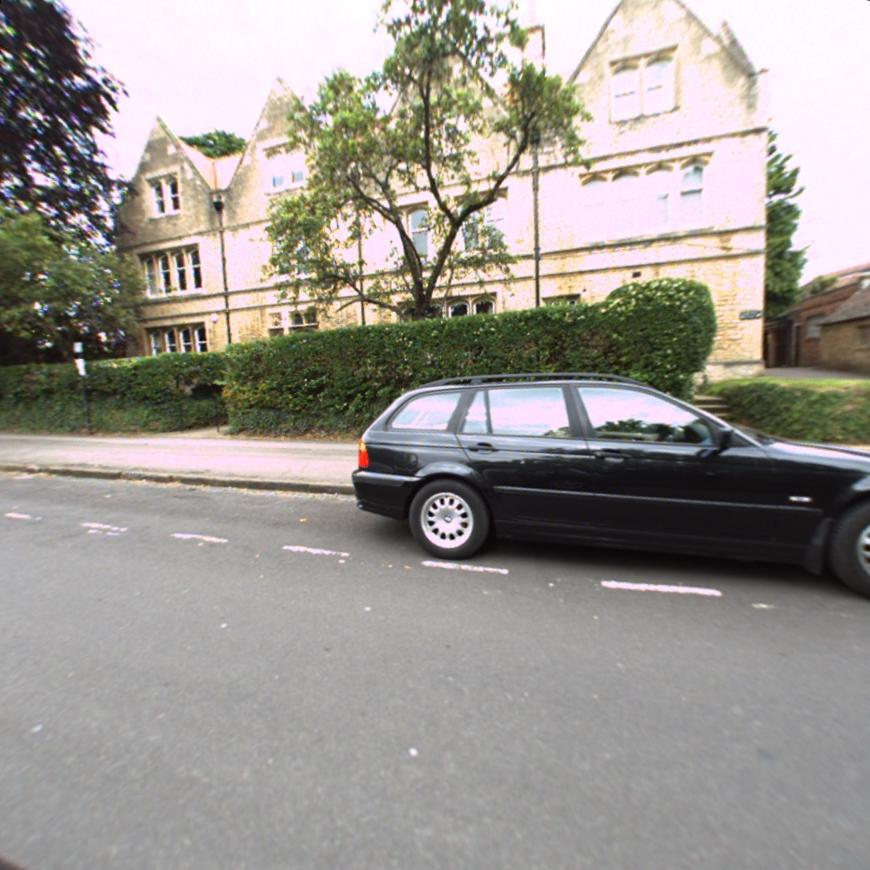
\includegraphics[width=0.12\linewidth]{ims_res/snow/q2/NetVLAD_our.jpg}}\hfill
%	\fcolorbox{red}{red}{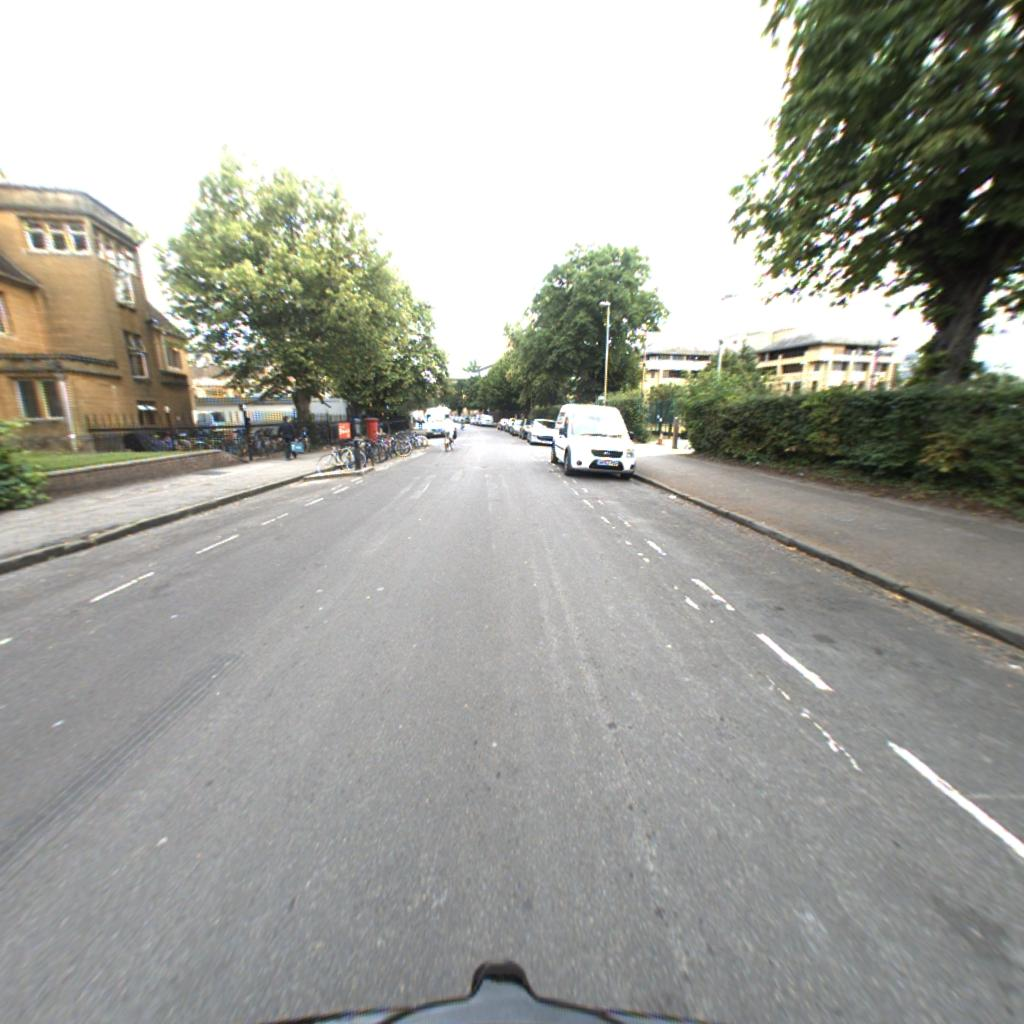
\includegraphics[width=0.12\linewidth]{ims_res/snow/q2/NetVLAD.jpg}}\hfill
%	\fcolorbox{red}{red}{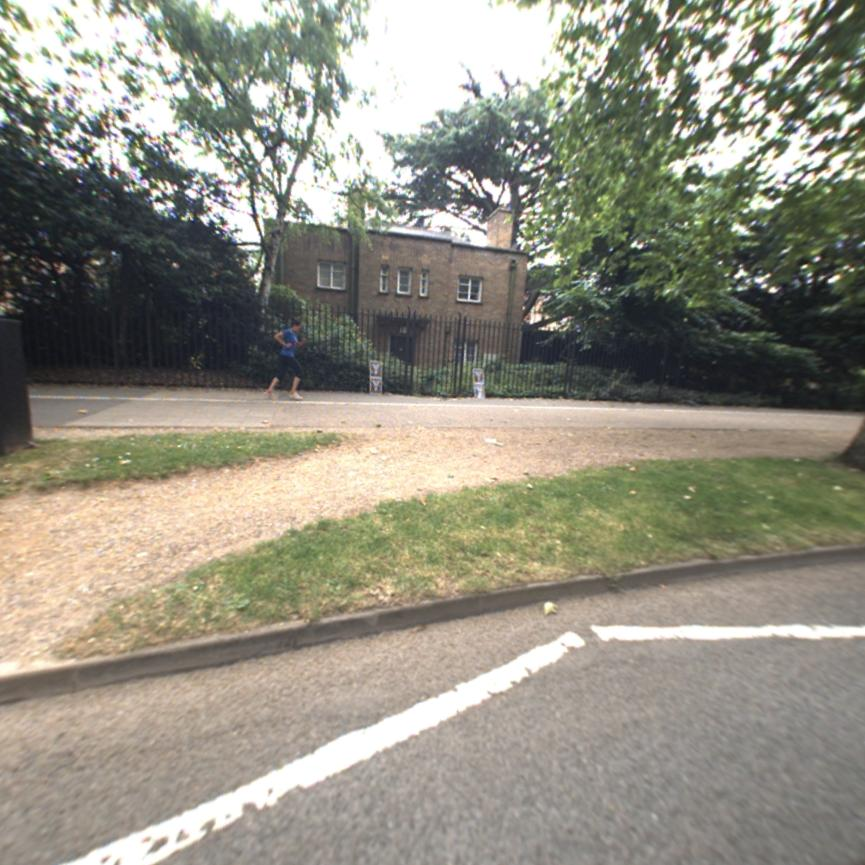
\includegraphics[width=0.12\linewidth]{ims_res/snow/q2/MAC_our.jpg}}\hfill
%	\fcolorbox{red}{red}{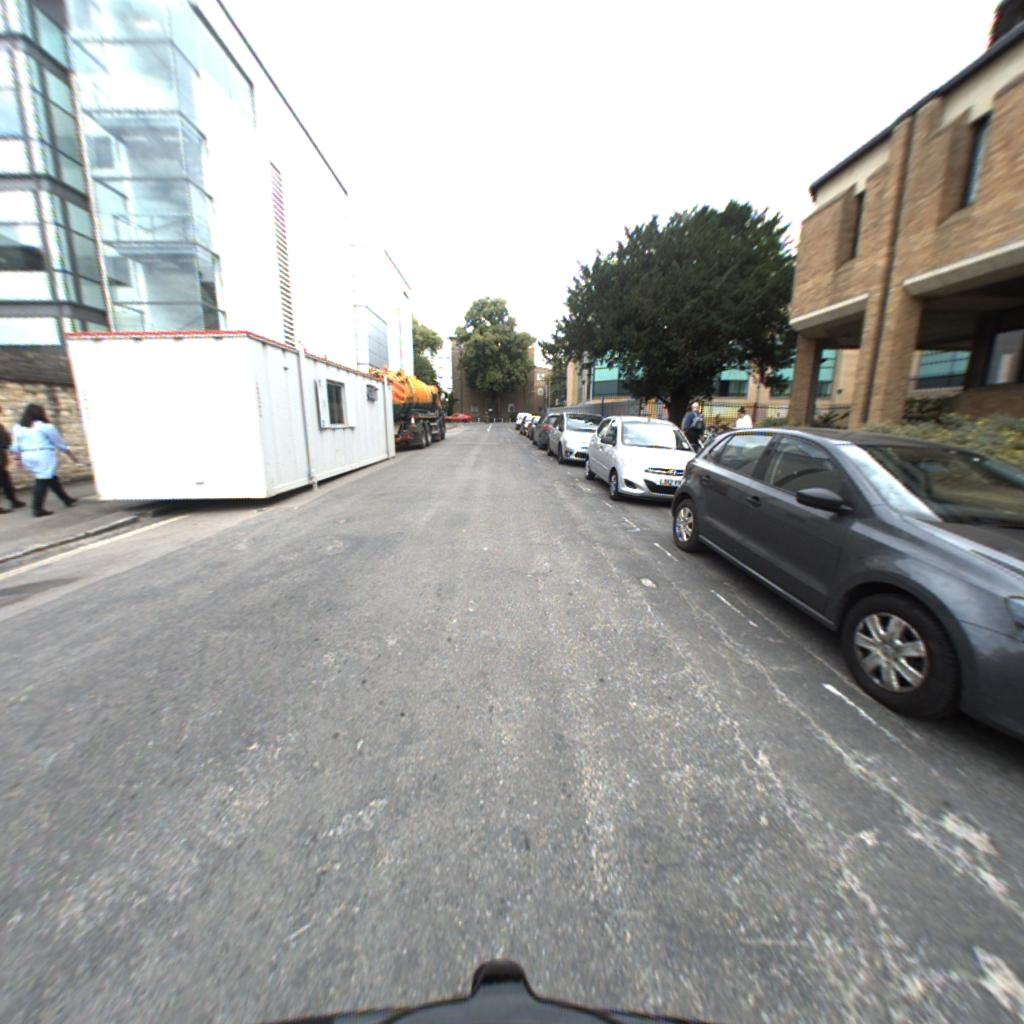
\includegraphics[width=0.12\linewidth]{ims_res/snow/q2/MAC.jpg}}
%	
%	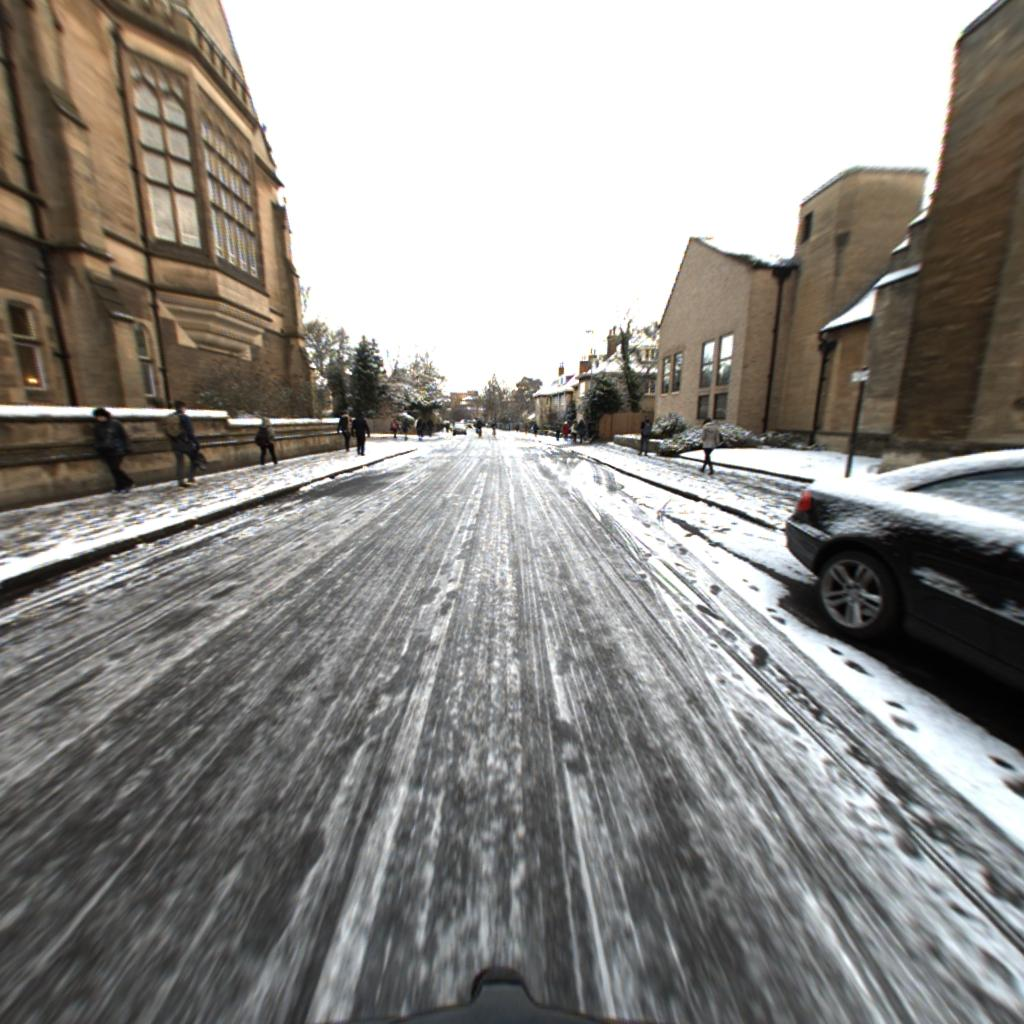
\includegraphics[width=0.12\linewidth]{ims_res/snow/q3/Q.jpg}\hfill
%	\fcolorbox{green}{green}{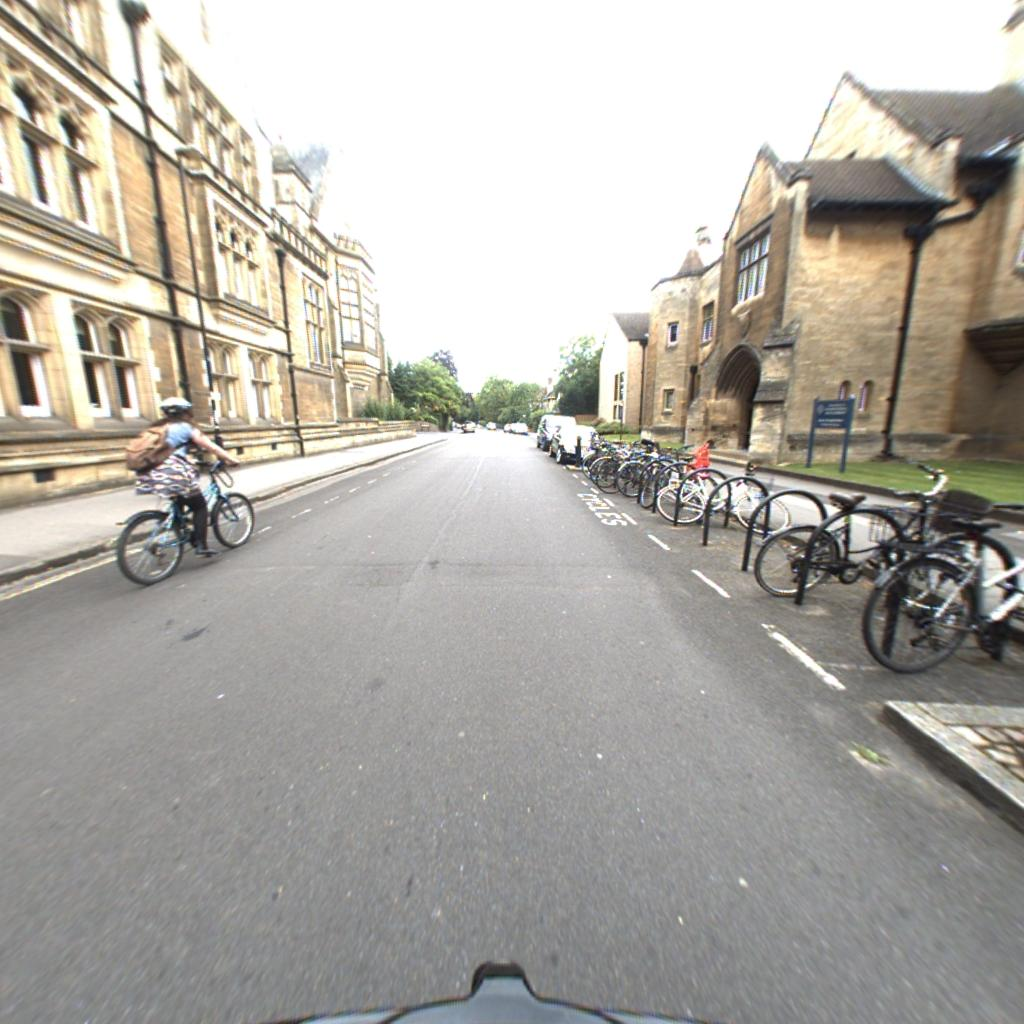
\includegraphics[width=0.12\linewidth]{ims_res/snow/q3/NetVLAD_our.jpg}}\hfill
%	\fcolorbox{red}{red}{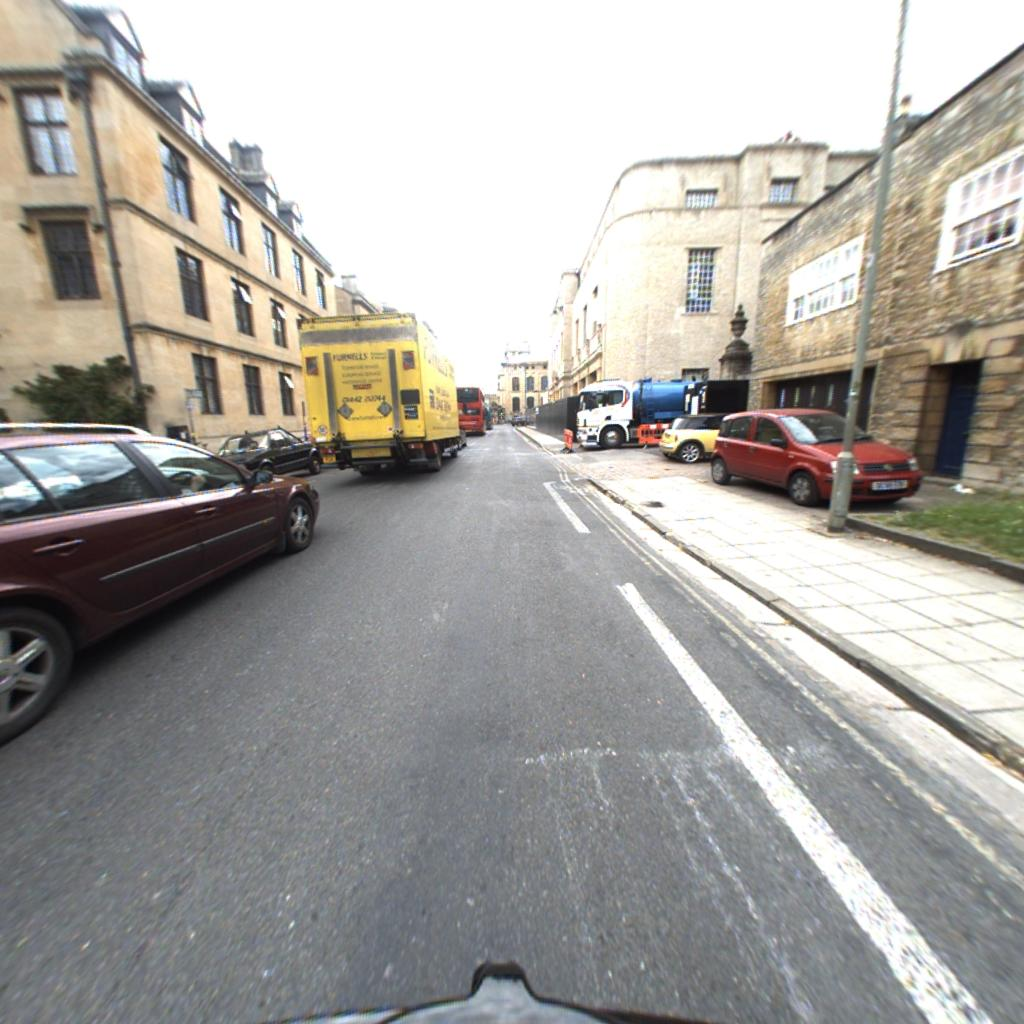
\includegraphics[width=0.12\linewidth]{ims_res/snow/q3/NetVLAD.jpg}}\hfill
%	\fcolorbox{red}{red}{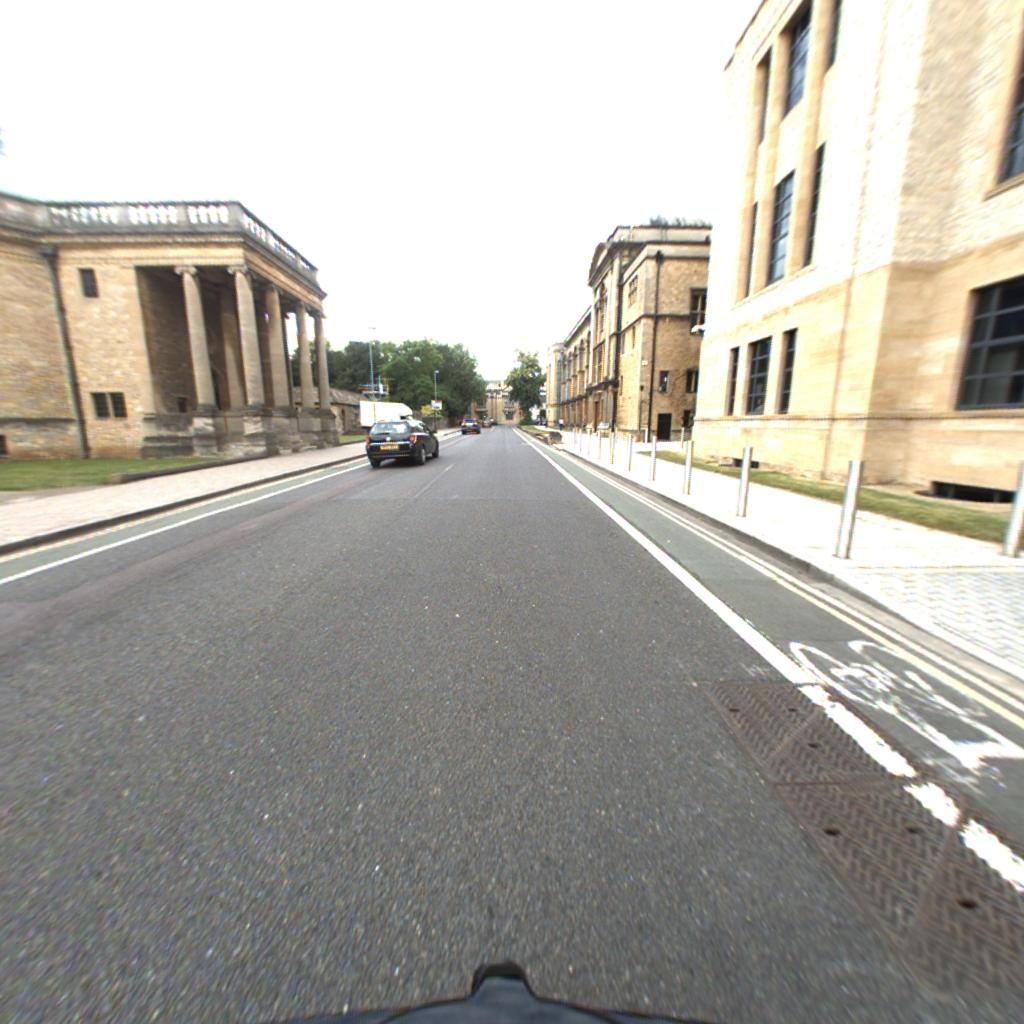
\includegraphics[width=0.12\linewidth]{ims_res/snow/q3/MAC_our.jpg}}\hfill
%	\fcolorbox{red}{red}{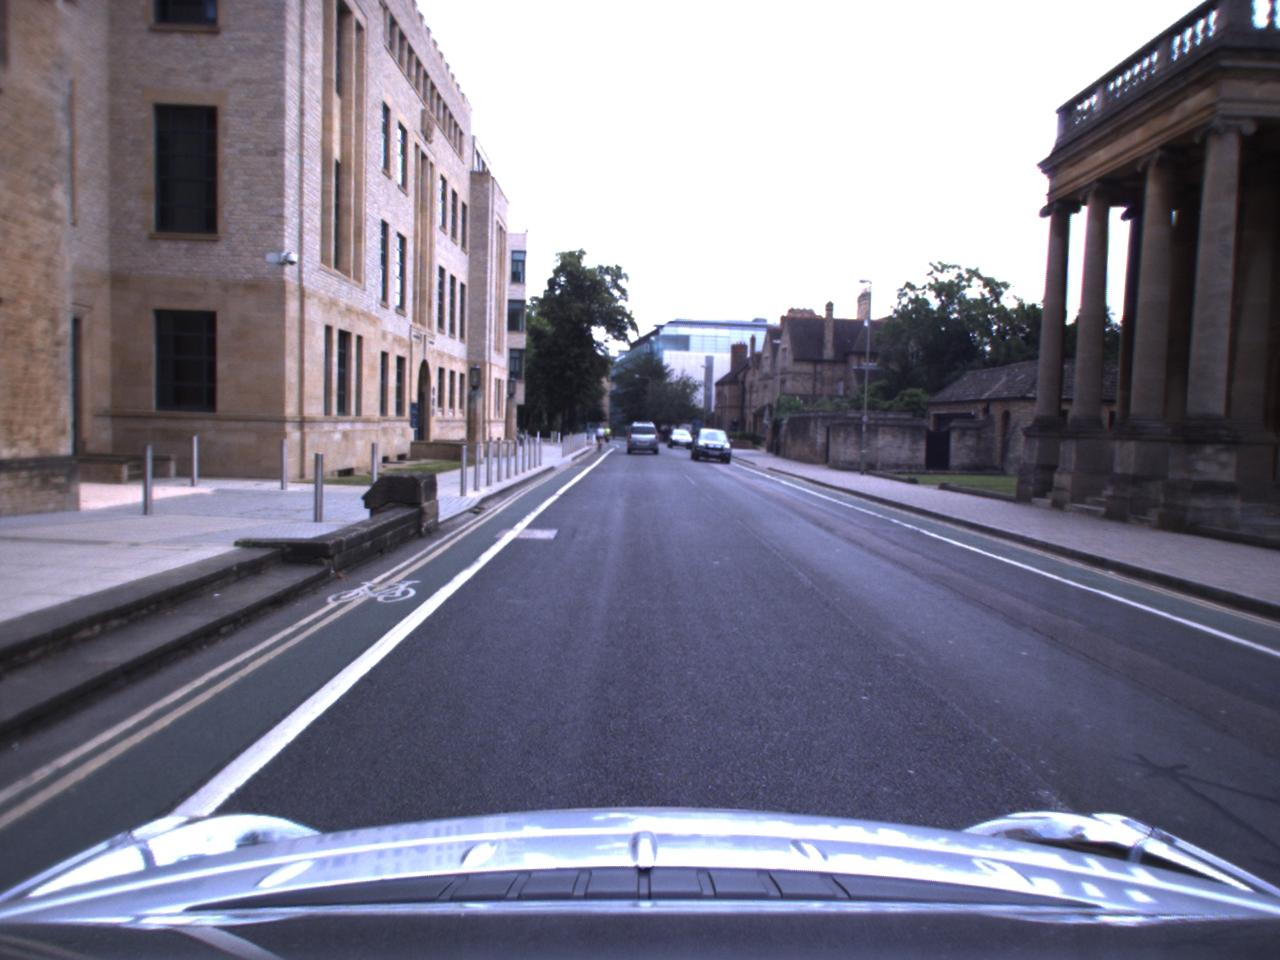
\includegraphics[width=0.12\linewidth]{ims_res/snow/q3/MAC.jpg}}
%	
%	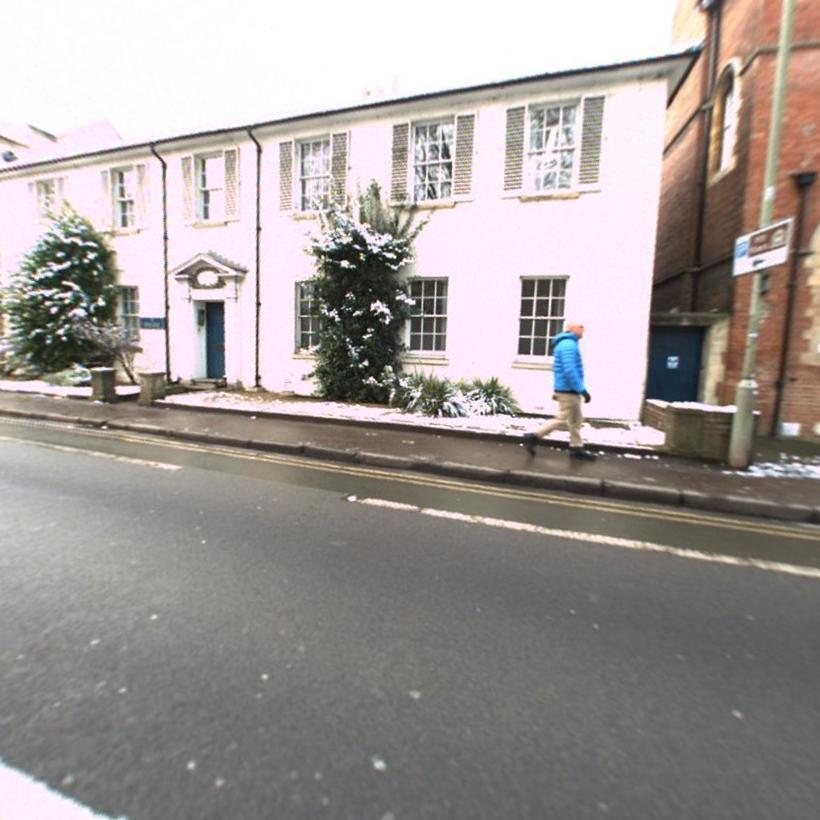
\includegraphics[width=0.12\linewidth]{ims_res/snow/q4/Q.jpg}\hfill
%	\fcolorbox{green}{green}{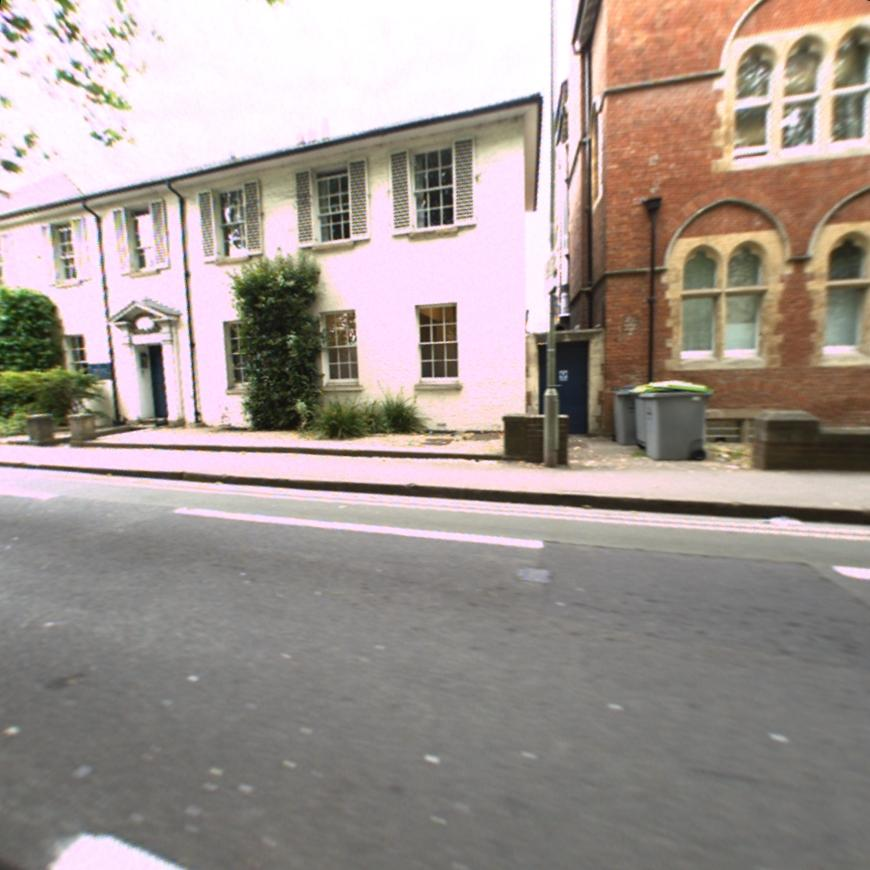
\includegraphics[width=0.12\linewidth]{ims_res/snow/q4/NetVLAD_our.jpg}}\hfill
%	\fcolorbox{green}{green}{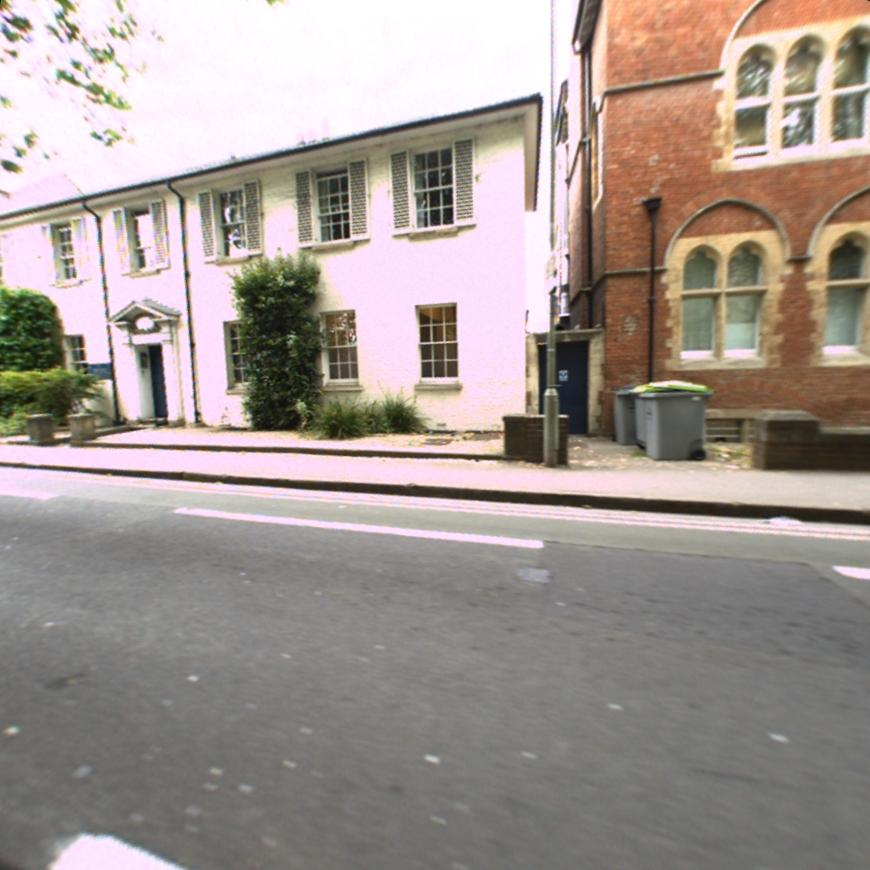
\includegraphics[width=0.12\linewidth]{ims_res/snow/q4/NetVLAD.jpg}}\hfill
%	\fcolorbox{green}{green}{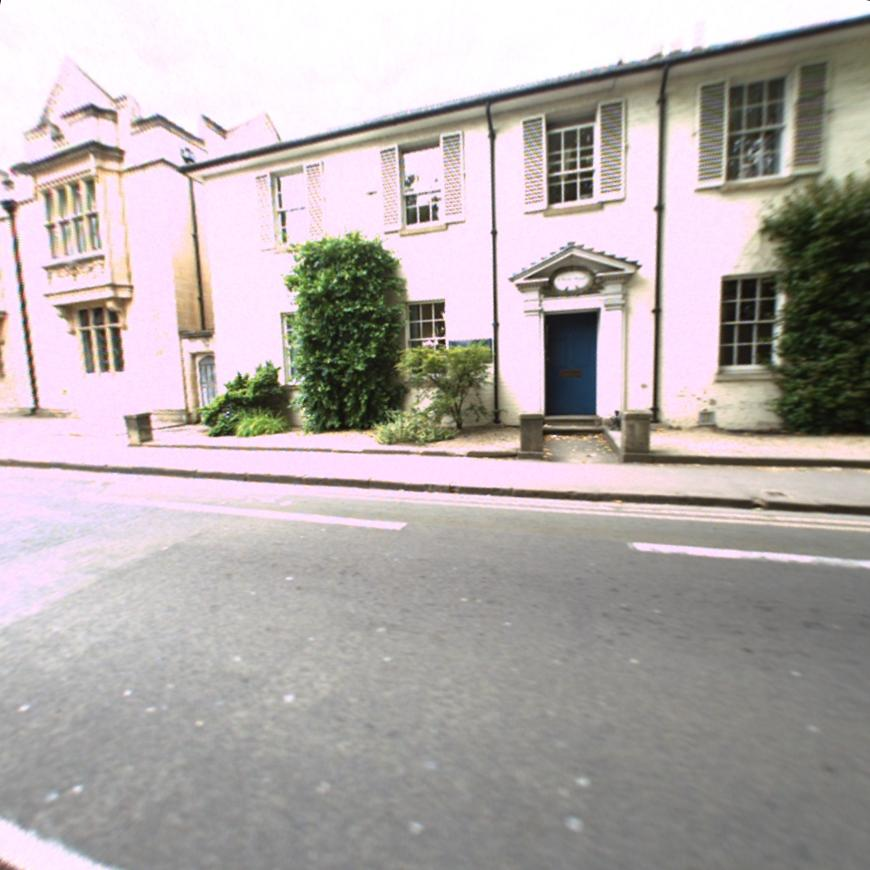
\includegraphics[width=0.12\linewidth]{ims_res/snow/q4/MAC_our.jpg}}\hfill
%	\fcolorbox{red}{red}{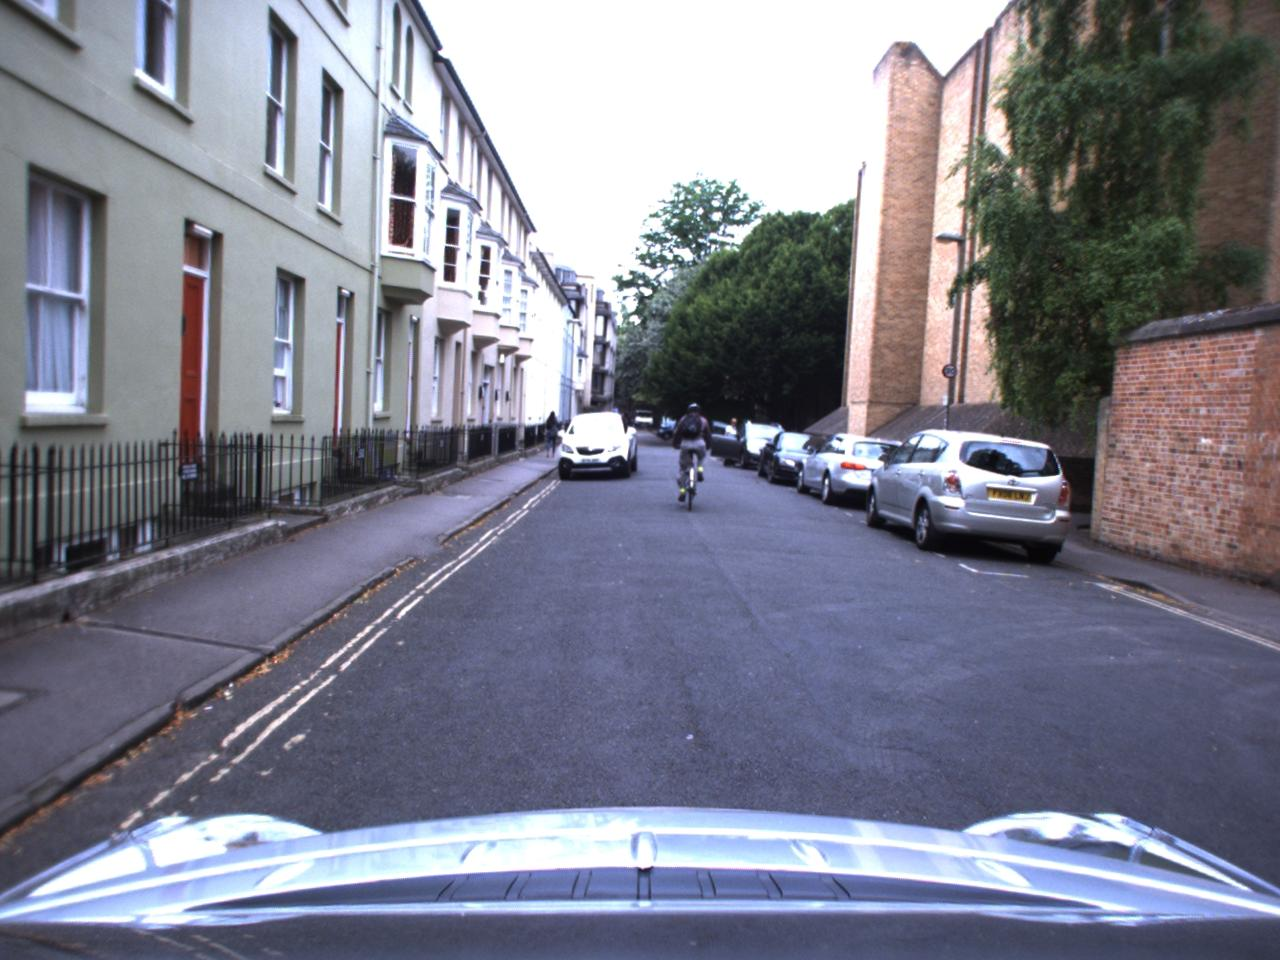
\includegraphics[width=0.12\linewidth]{ims_res/snow/q4/MAC.jpg}}
%\end{frame}

\begin{frame}{Results: long-term localization}
	\begin{minipage}{0.27\linewidth}
			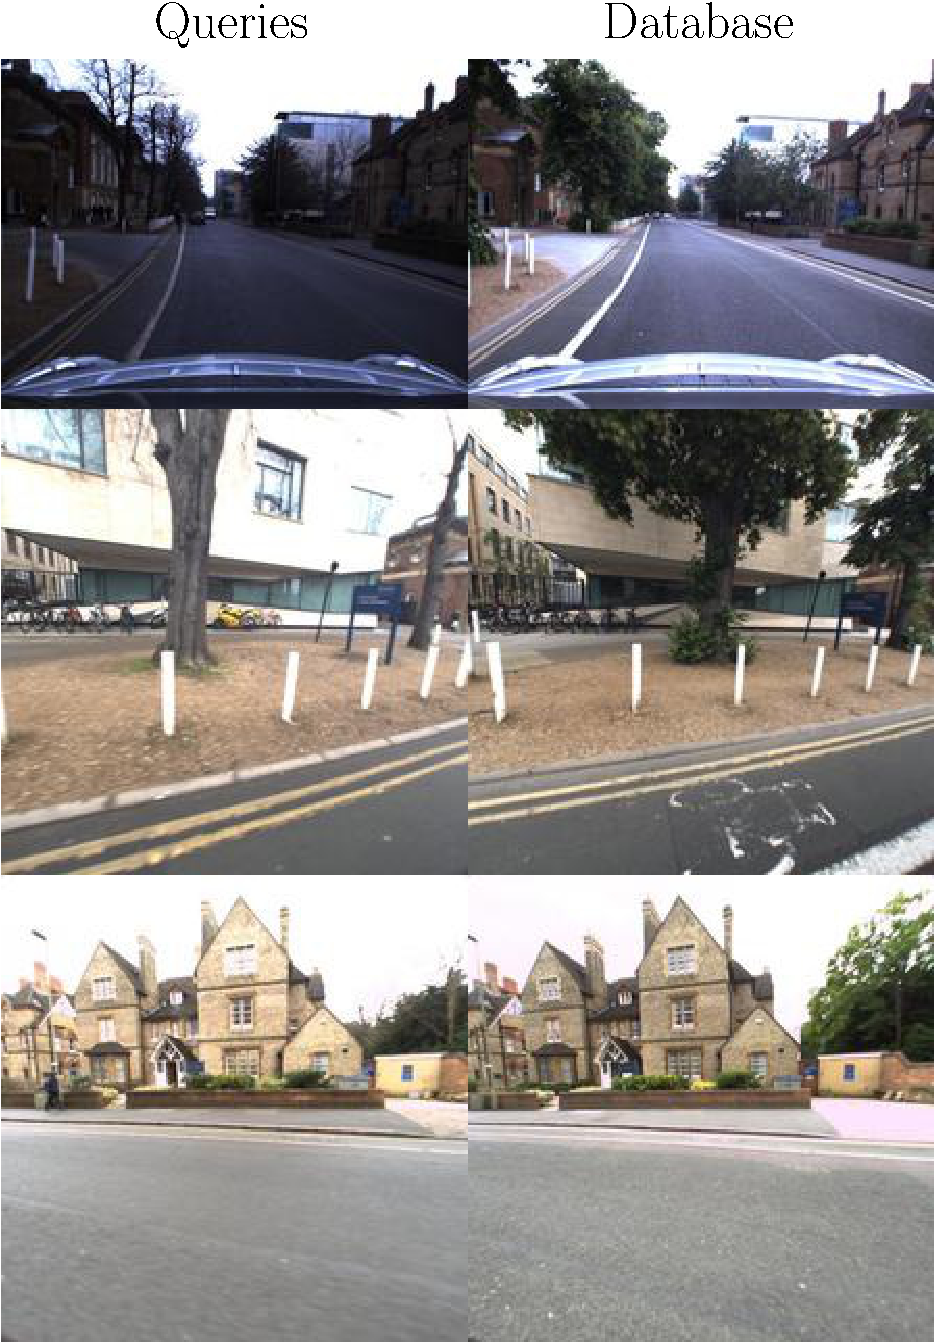
\includegraphics[width=\linewidth]{vect/res/dataset/lt_ex}
			\vfill

			{\scriptsize Example of queries and nearest image in the database.}
	\end{minipage}\hfill
	\begin{minipage}{0.49\linewidth}
		\centering
		\begin{figure}
			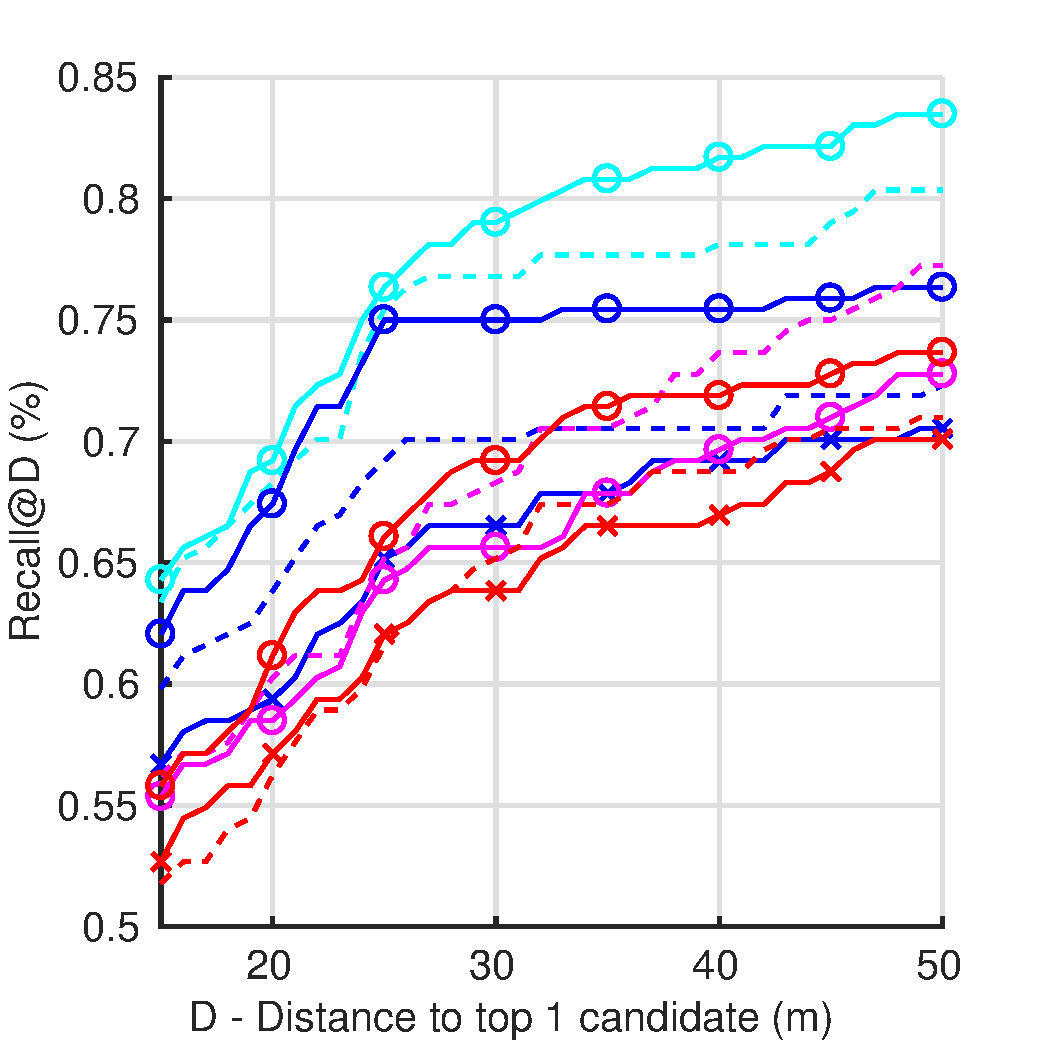
\includegraphics[width=0.9\linewidth]{vect/res/lt}
		\end{figure}
	\end{minipage}\hfill
	\begin{minipage}{0.2\linewidth}
			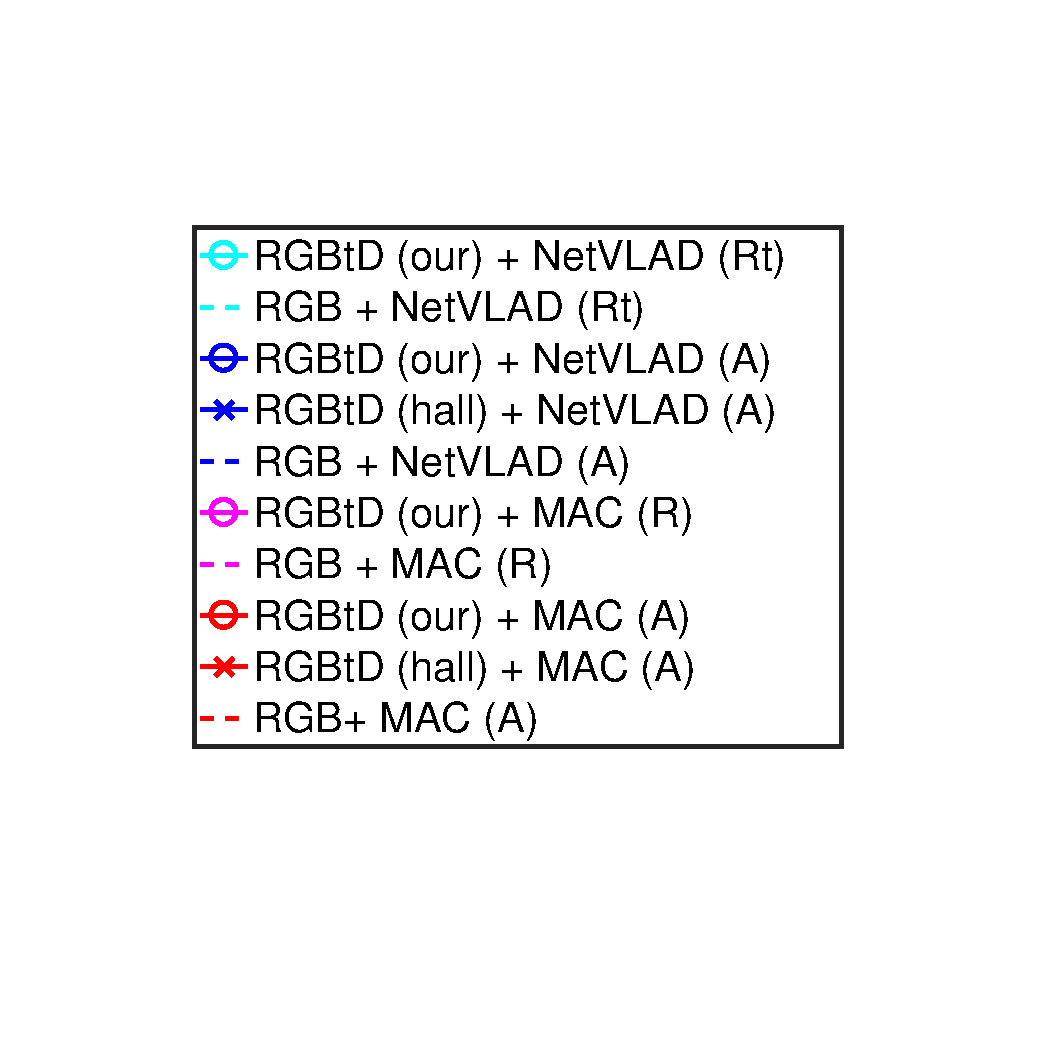
\includegraphics[trim={90 140 95 100},clip,width=\linewidth]{vect/res/legend}	
			\vspace{0.5cm}	
			{\scriptsize
			Competitors:
			\begin{itemize}
				\item[\textbf{-{}-{}-}] Only RGB [RGB]
				\item[\textbf{-x-}] Hallucination network [RGBtD (Hall)]
				\item[\textbf{-o-}] Our proposal [RGBtD (our)]
			\end{itemize}
			}
	\end{minipage}
\end{frame}

\begin{frame}{Results: cross-season localization}
	\begin{minipage}{0.27\linewidth}
			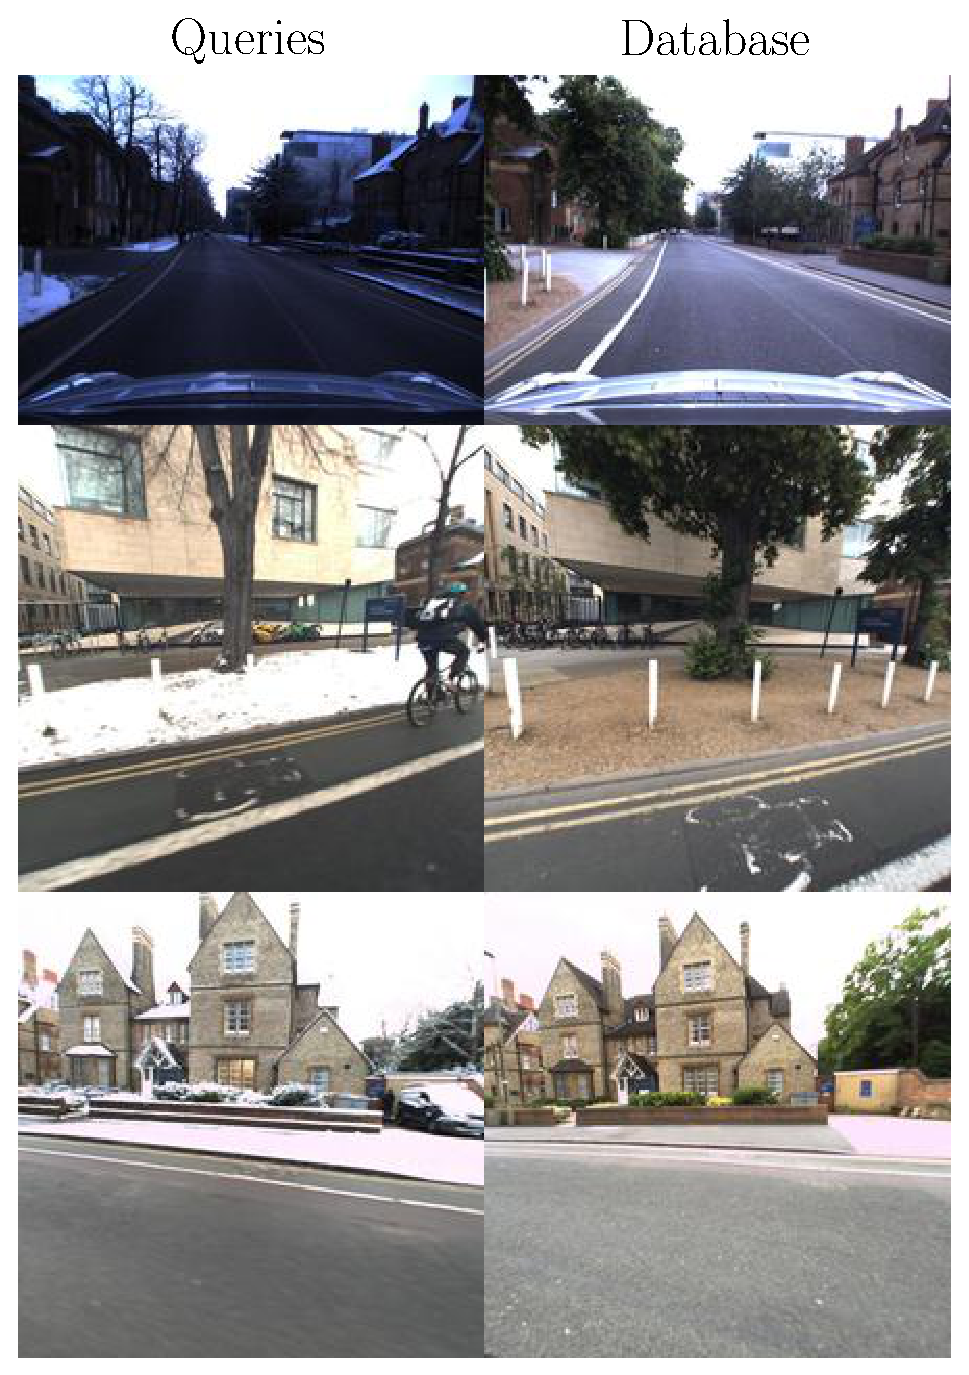
\includegraphics[width=\linewidth]{vect/res/dataset/snow_ex}
			\vfill

			{\scriptsize Example of queries and nearest image in the database.}
	\end{minipage}\hfill
	\begin{minipage}{0.49\linewidth}
		\centering
		\begin{figure}
			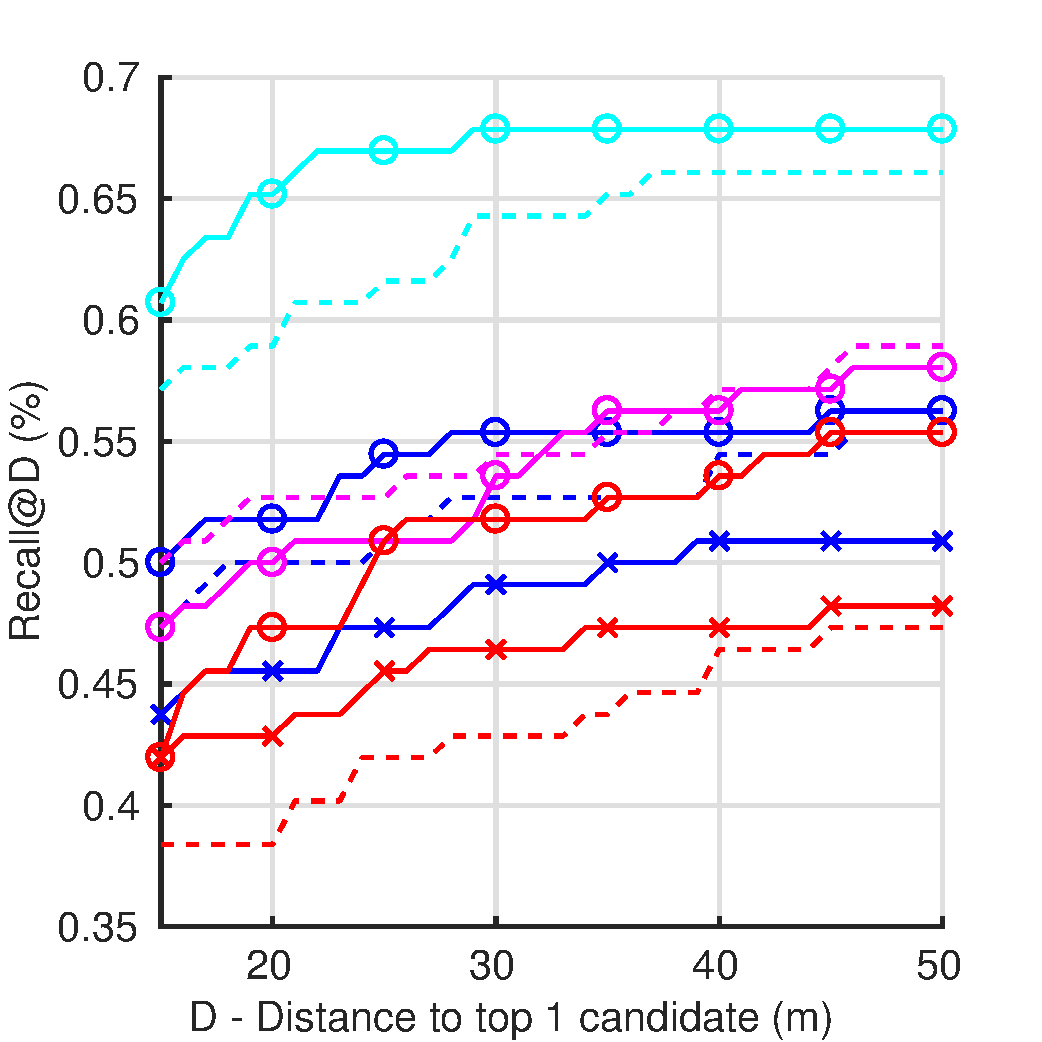
\includegraphics[width=0.9\linewidth]{vect/res/snow}
		\end{figure}
	\end{minipage}\hfill
	\begin{minipage}{0.2\linewidth}
			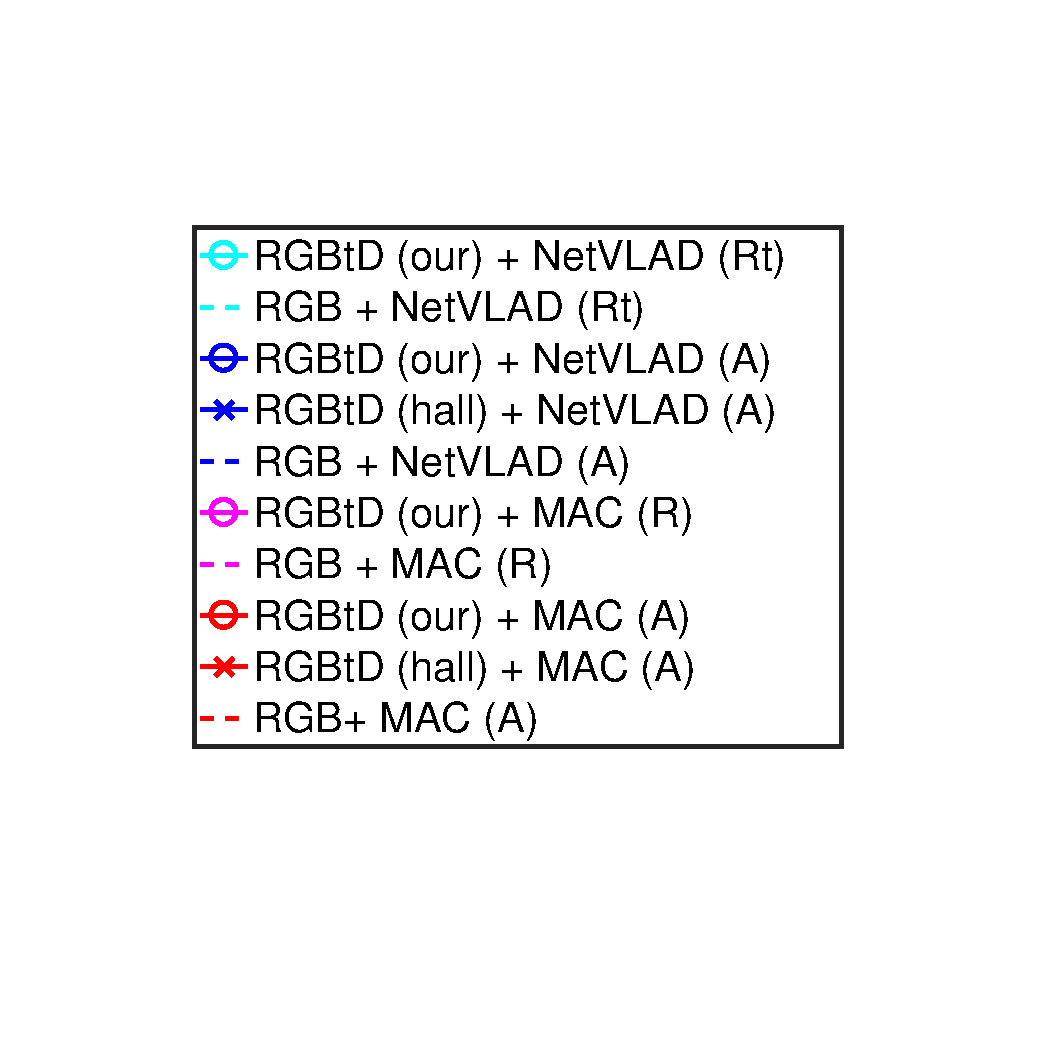
\includegraphics[trim={90 140 95 100},clip,width=\linewidth]{vect/res/legend}	
			\vspace{0.5cm}	
			{\scriptsize
			Competitors:
			\begin{itemize}
				\item[\textbf{-{}-{}-}] Only RGB [RGB]
				\item[\textbf{-x-}] Hallucination network [RGBtD (Hall)]
				\item[\textbf{-o-}] Our proposal [RGBtD (our)]
			\end{itemize}
			}
	\end{minipage}
\end{frame}

\begin{frame}{Failure case: Night to day}
	\begin{minipage}{0.27\linewidth}
			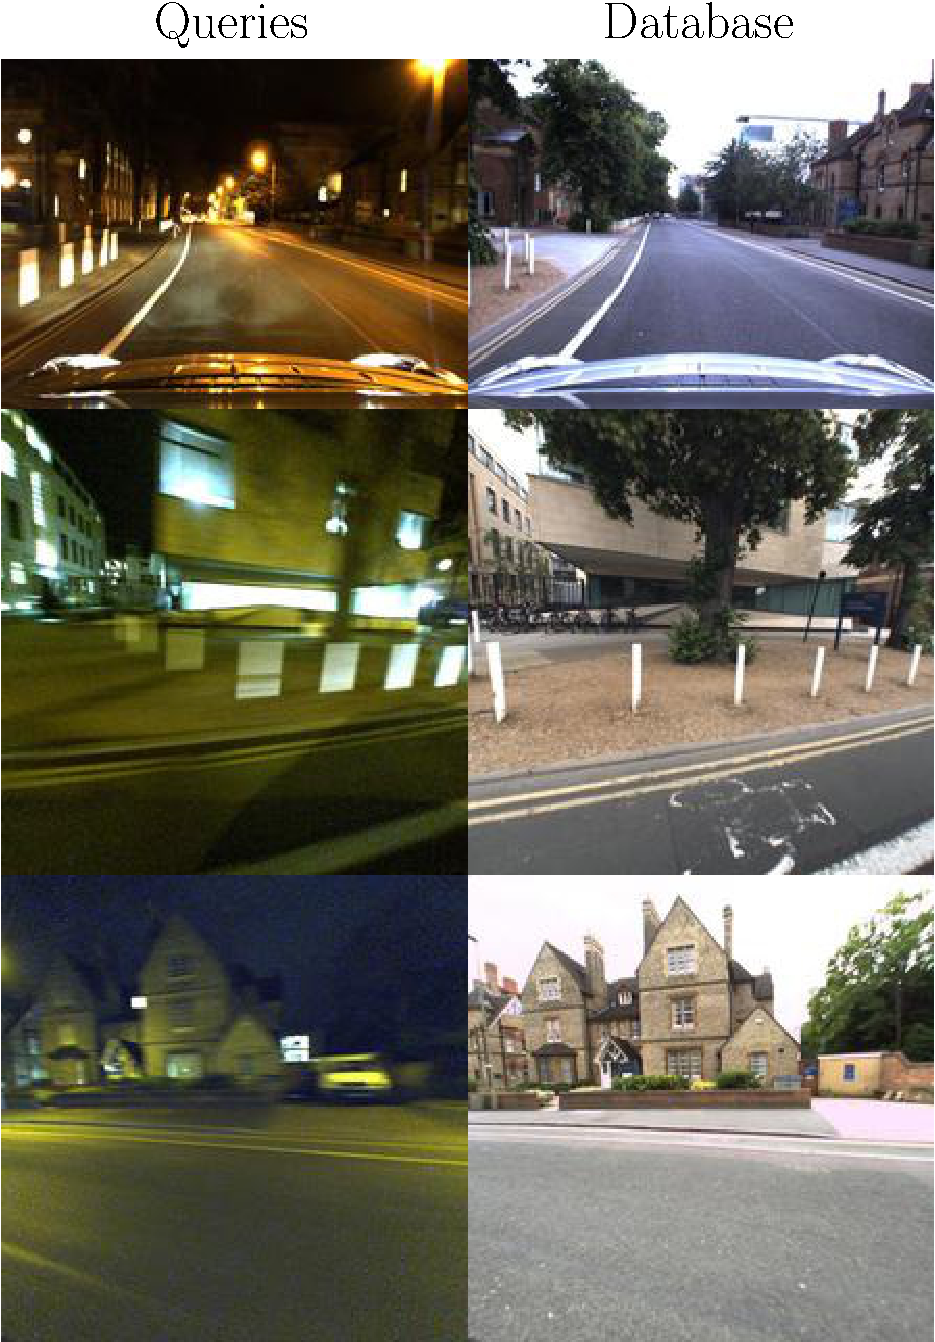
\includegraphics[width=\linewidth]{vect/res/dataset/night_ex}
			\vfill

			{\scriptsize Example of queries and nearest image in the database.}
	\end{minipage}\hfill
	\begin{minipage}{0.49\linewidth}
		\centering
		\begin{figure}
			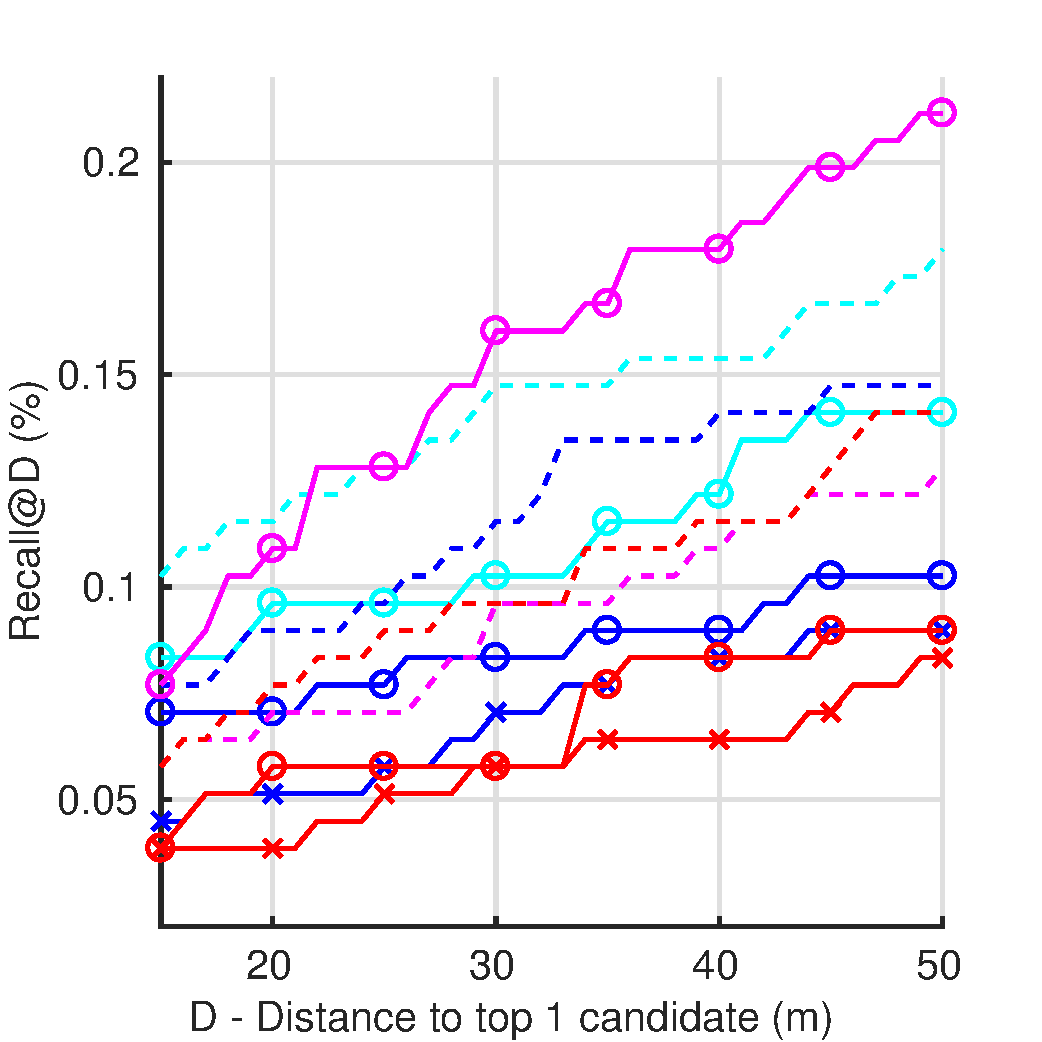
\includegraphics[width=0.9\linewidth]{vect/res/night}
		\end{figure}
	\end{minipage}\hfill
	\begin{minipage}{0.2\linewidth}
			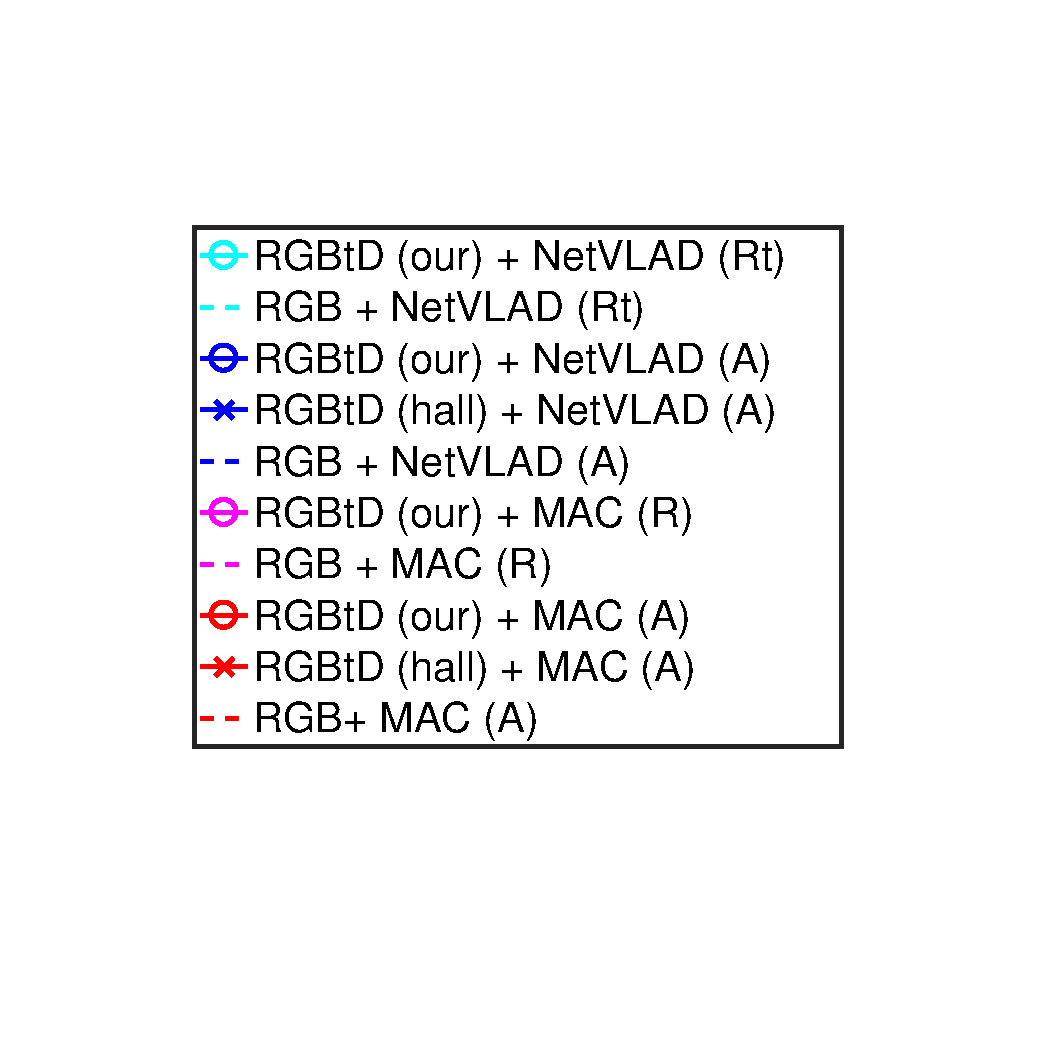
\includegraphics[trim={90 140 95 100},clip,width=\linewidth]{vect/res/legend}	
			\vspace{0.5cm}	
			{\scriptsize
			Competitors:
			\begin{itemize}
				\item[\textbf{-{}-{}-}] Only RGB [RGB]
				\item[\textbf{-x-}] Hallucination network [RGBtD (Hall)]
				\item[\textbf{-o-}] Our proposal [RGBtD (our)]
			\end{itemize}
			}
	\end{minipage}
\end{frame}


\begin{frame}{Improving night to day localization}
	\begin{minipage}{0.80\linewidth}
	\begin{figure}
		\centering
		\begin{minipage}{0.74\linewidth}
			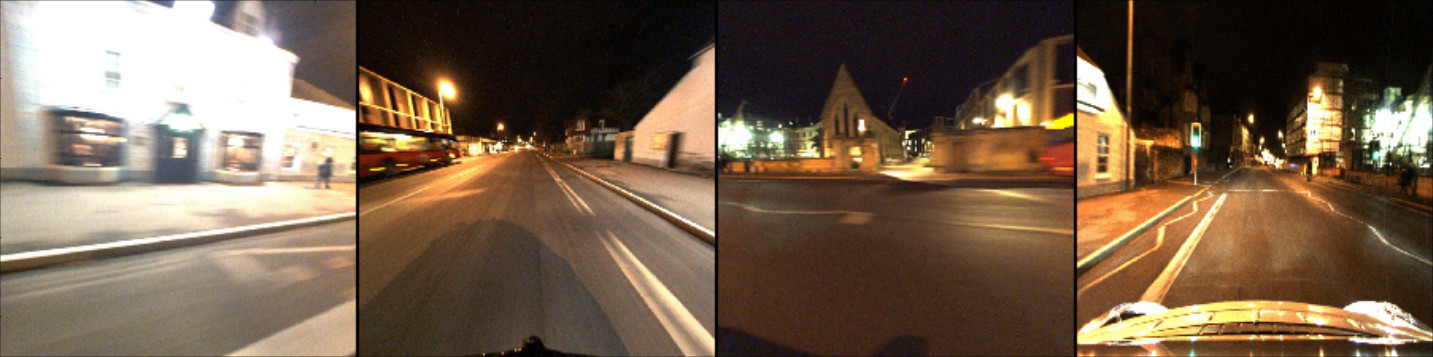
\includegraphics[width=\linewidth]{im/res/night_input}
		\end{minipage}
		\begin{minipage}{0.25\linewidth}
			\raggedright \footnotesize
			{Night images that serve as input for the generative network}
		\end{minipage}
	\end{figure}
	\vspace{-0.5cm}
	\begin{figure}
		\centering
		\begin{minipage}{0.74\linewidth}
			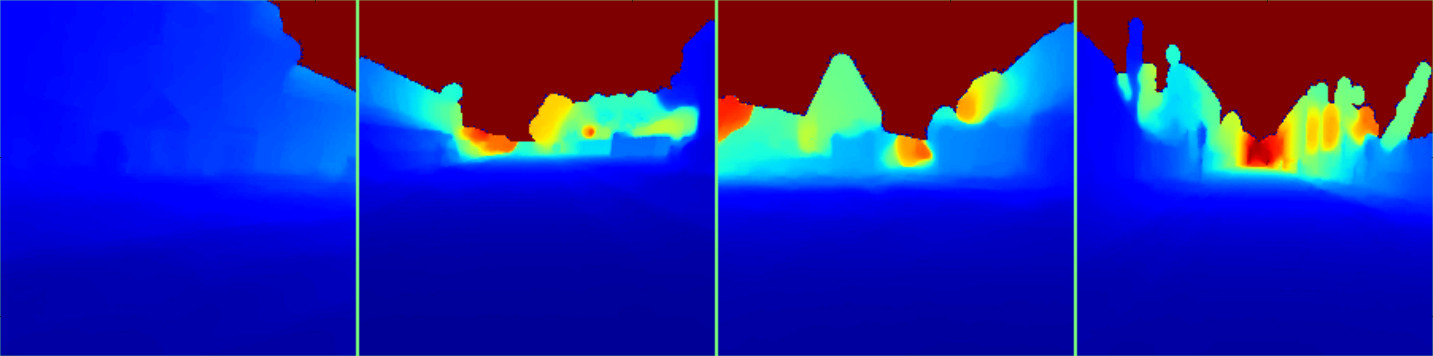
\includegraphics[width=\linewidth]{im/res/night_gt}
		\end{minipage}
		\begin{minipage}{0.25\linewidth}
			\raggedright \footnotesize
			{Ground truth depth maps}
		\end{minipage}
	\end{figure}	
	\vspace{-0.5cm}
	\begin{figure}
		\centering
		\begin{minipage}{0.74\linewidth}
			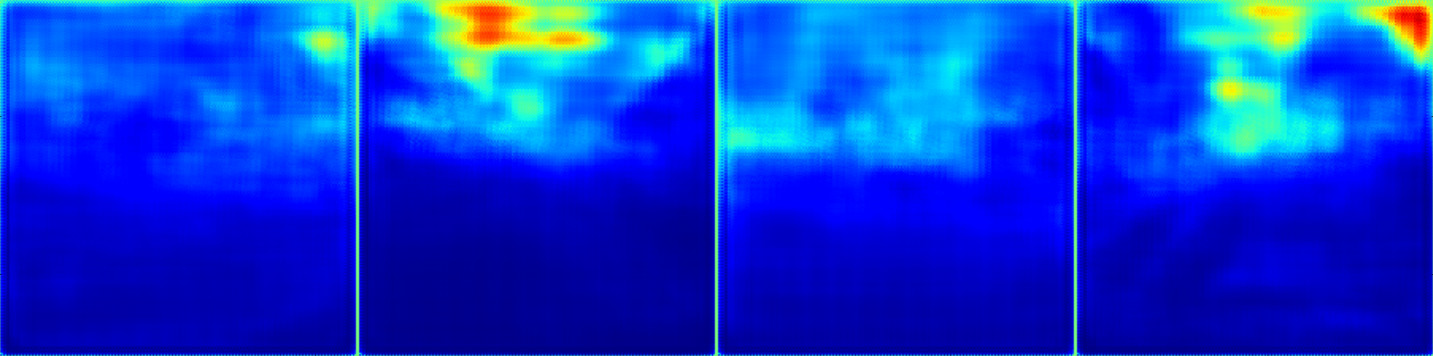
\includegraphics[width=\linewidth]{im/res/night_noft}
		\end{minipage}
		\begin{minipage}{0.25\linewidth}
			\raggedright \footnotesize
			{Generated depth maps}
		\end{minipage}
	\end{figure}
	\end{minipage}
	\vfill

	\textbf{Our network is \textit{not able} to generate proper depth maps from night images.}
\end{frame}

\begin{frame}{Recall - Training policy}
	\begin{minipage}{0.6\linewidth}
		\centering
		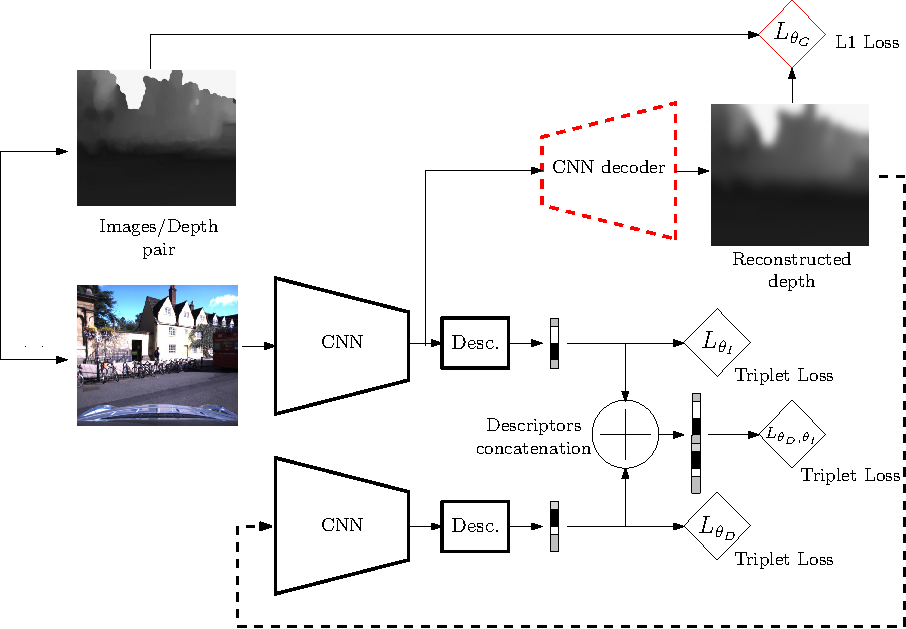
\includegraphics[width=\linewidth]{vect/method/fig3/6d}	
	\end{minipage}\hfill
	\begin{minipage}{0.3\linewidth}
		\raggedright
		Thanks to the design of our method, we can improve generation performances of the decoder without impacting the descriptors networks.
		
		\uncover<2>{
		We fine tune our system with pairs of night image/depth map.
		\vspace{0.5cm}
		
		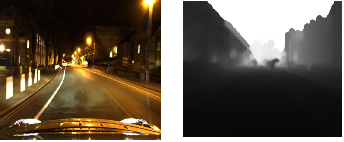
\includegraphics[width=\linewidth]{vect/res/fig1/night_pair}
		}
	\end{minipage}			
\end{frame}

\begin{frame}{Improving night to day localization}
\centering
\begin{minipage}{0.7\linewidth}
	\centering
	
	\begin{figure}
		\centering
		\begin{minipage}{0.74\linewidth}
			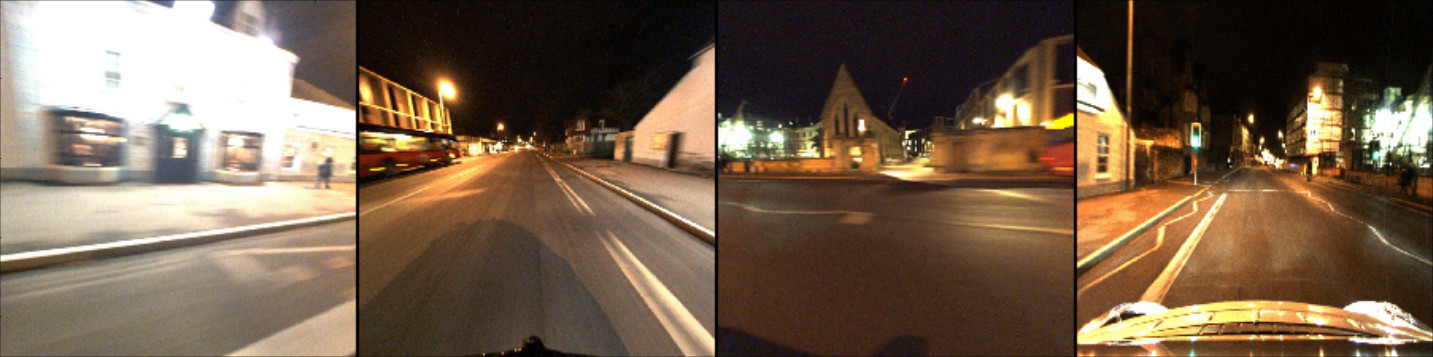
\includegraphics[width=\linewidth]{im/res/night_input}
		\end{minipage}
		\begin{minipage}{0.21\linewidth}
			\raggedright \footnotesize
			Night images that serve as input for the generative network
		\end{minipage}
	\end{figure}
	\vspace{-0.5cm}
	\begin{figure}
		\centering
		\begin{minipage}{0.74\linewidth}
			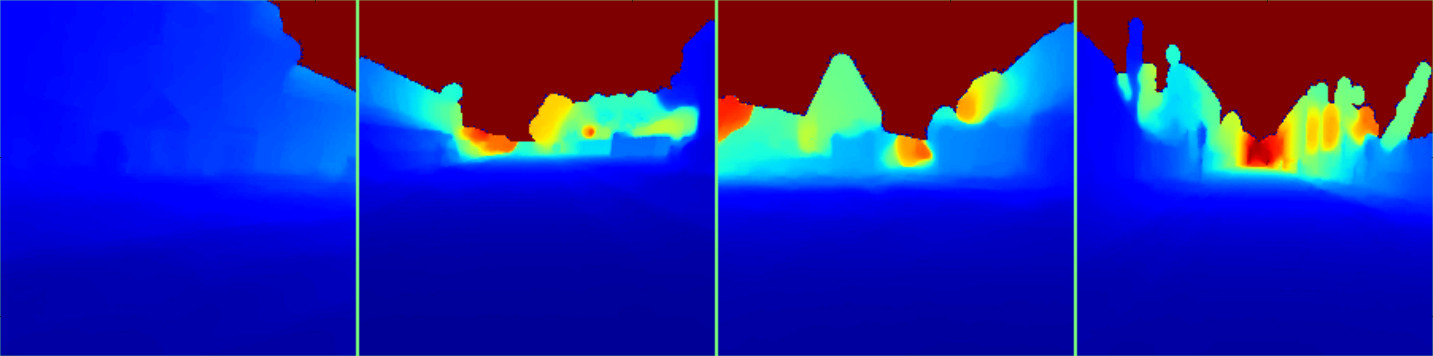
\includegraphics[width=\linewidth]{im/res/night_gt}
		\end{minipage}
		\begin{minipage}{0.21\linewidth}
			\raggedright \footnotesize
			Ground truth depth maps
		\end{minipage}
	\end{figure}	
	\vspace{-0.5cm}
	\begin{figure}
		\centering
		\begin{minipage}{0.74\linewidth}
			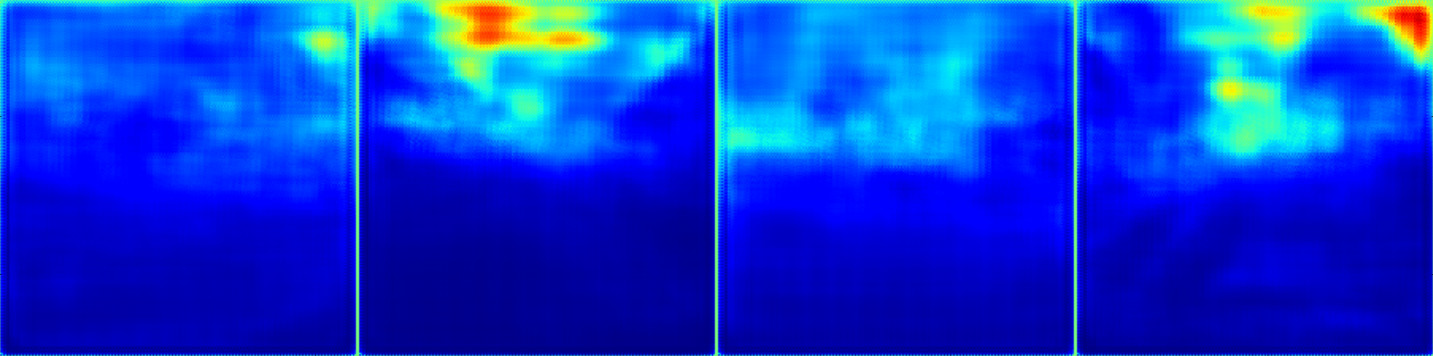
\includegraphics[width=\linewidth]{im/res/night_noft}
		\end{minipage}
		\begin{minipage}{0.21\linewidth}
			\raggedright \footnotesize
			Generated depth maps
		\end{minipage}
	\end{figure}
		\vspace{-0.5cm}
		\begin{figure}
			\centering
			\begin{minipage}{0.74\linewidth}
				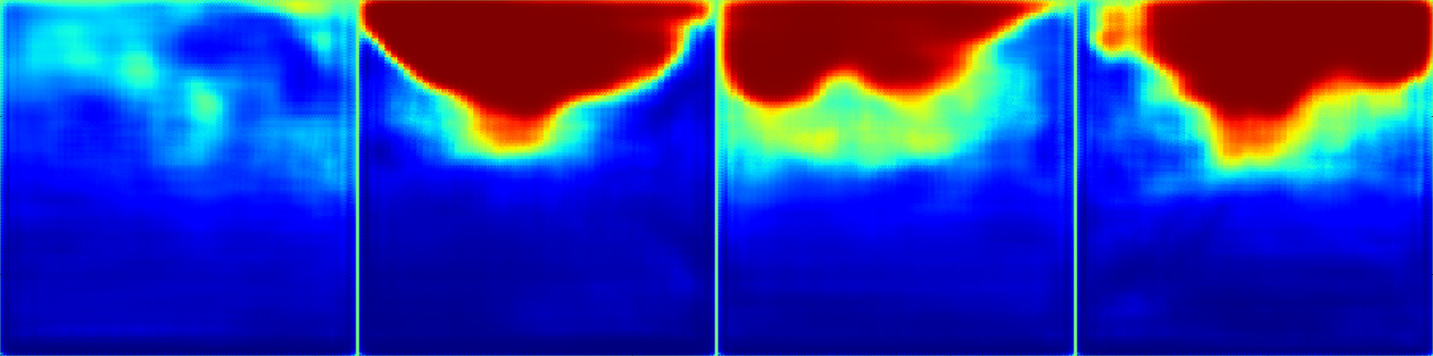
\includegraphics[width=\linewidth]{im/res/night_ft}
			\end{minipage}
			\begin{minipage}{0.21\linewidth}
				\raggedright \footnotesize
				Generated depth maps, with fine tuning
			\end{minipage}
		\end{figure}
\end{minipage}
\end{frame}

\begin{frame}{Results: Night to day (fine tuning)}
	\begin{minipage}{0.49\linewidth}
		\centering
		\begin{figure}
			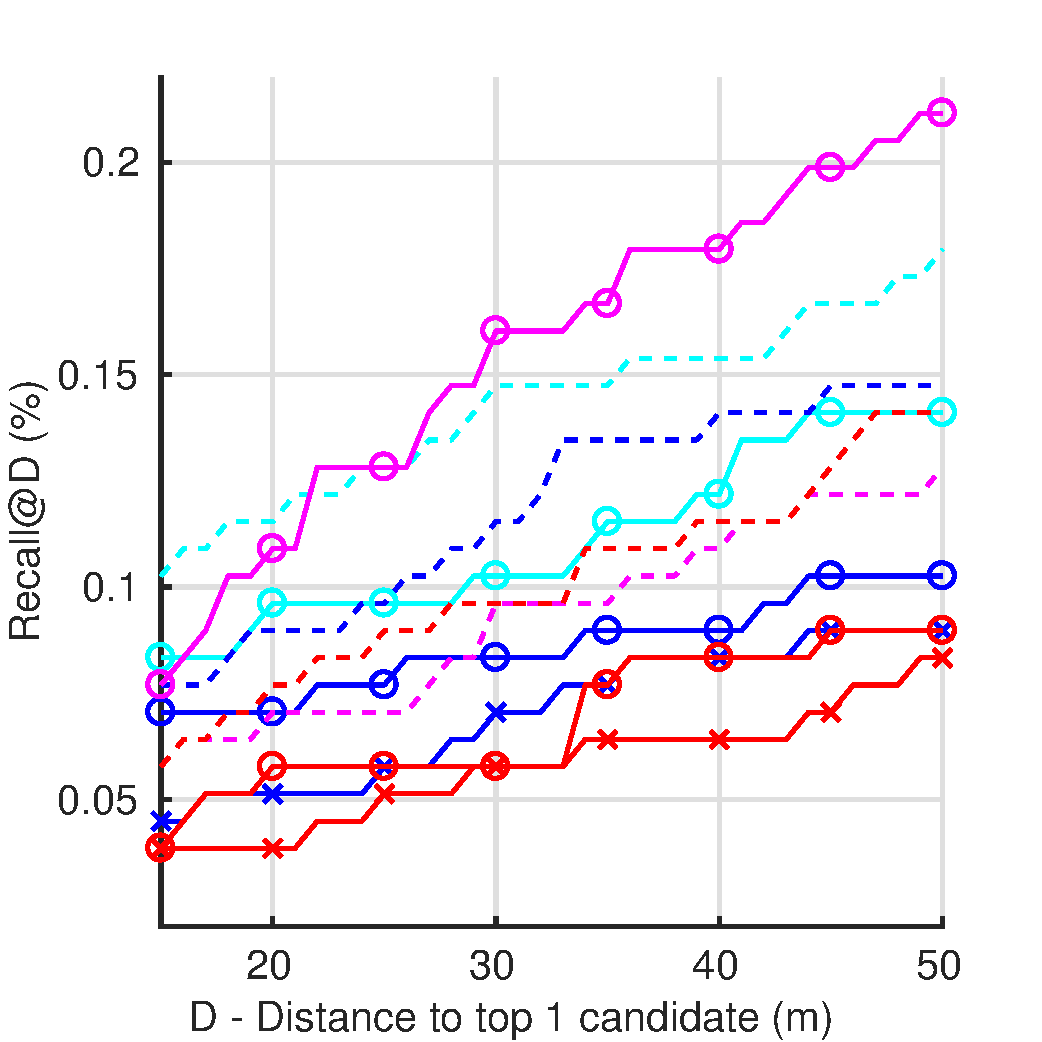
\includegraphics[width=0.9\linewidth]{vect/res/night}
			
			{Night vs daytime (w/o fine tuning)}
		\end{figure}
	\end{minipage}\hfill
	\begin{minipage}{0.49\linewidth}
		\centering
		\begin{figure}
			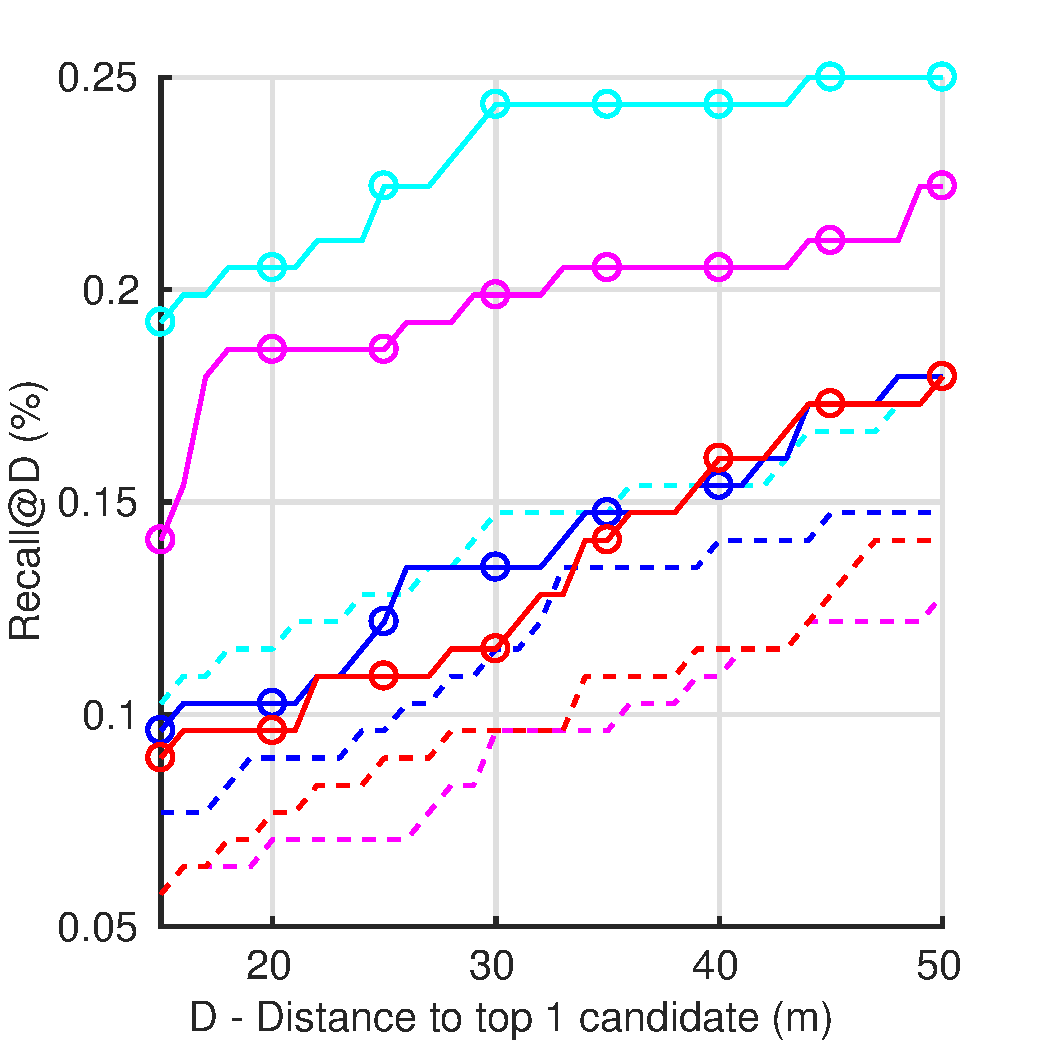
\includegraphics[width=0.9\linewidth]{vect/res/nightft}
			
			{Night vs daytime (w/ fine tuning)}
		\end{figure}
	\end{minipage}
	\vfill 
	
	{\small With fine tuning with a small amount of data, we are able to nearly double localization performances.}
\end{frame}